\documentclass[10pt,a4paper]{article}
%\documentclass[aps,prl]{revtex4-1}
\usepackage[margin=1.7cm,footskip=0.35cm,includefoot]{geometry}% spremenimo sirine robov
\usepackage{floatrow}
\usepackage{hyperref}
\usepackage{amsmath}
\usepackage{fullpage}
\usepackage{amsfonts}
\usepackage{amssymb}
\usepackage{lmodern}
\usepackage{url}
\usepackage[labelformat=simple,font=small]{subcaption}
\usepackage[font=small]{caption}
%\usepackage{subcaption}
\usepackage[multiple]{footmisc}
\usepackage[]{units}
\usepackage{bm}
\usepackage{fancyhdr}
% \pagestyle{fancy}
\fancyhf{}
\fancyhead[R]{\thepage}
%\usepackage[demo]{graphicx}
\usepackage{graphicx}
\usepackage{mhchem}
\newcommand{\iu}{{i\mkern1mu}}

\addtolength\hoffset{0.5cm}%horizontalni premik
%vse pametne funkcije ki jih lahko rabimo (lahko tudi kopiras direktno zraven)
\setlength{\parindent}{0pt}%ni pomika za paragrafe
\setlength{\parskip}{0.75ex}%med paragrafi je malo lufta

\usepackage[pdftex]{graphicx}%za slike: predvidimo da bomo klicali pdflatex.

\usepackage{amsmath}
\usepackage{amsfonts}
\usepackage{mathrsfs}
\usepackage[usenames]{color}
\usepackage[slovene]{babel}
\usepackage[utf8]{inputenc}%to omogoca uporabo sumnikov. Brez tega rabis \v{c}, \v{s}, \v{z} in vse ostalo.

%nekaj koristnih funkcij.
\newcommand{\HRule}{\rule{\linewidth}{0.5mm}}   %debela črta čez celo stran

\newcommand{\ve}[1]{\ensuremath{\mathbf{#1}}} % for vectors
\newcommand{\gv}[1]{\ensuremath{\mbox{\boldmath$ #1 $}}} 
% for vectors of Greek letters
\newcommand{\uv}[1]{\ensuremath{\mathbf{\hat{#1}}}} % for unit vector
\newcommand{\abs}[1]{\left| #1 \right|} % for absolute value

\renewcommand{\Re}{\mathop{\rm Re}}
\renewcommand{\Im}{\mathop{\rm Im}}
\newcommand{\Tr}{\mathop{\rm Tr}}
\newcommand{\dd}{\,\mathrm{d}}
\newcommand{\ddd}{\mathrm{d}}
\newcommand{\ii}{\mathrm{i}}
\newcommand{\lag}{\mathcal{L}\!}
\newcommand{\ham}{\mathcal{H}\!}
\newcommand{\four}[1]{\mathcal{F}\!\left(#1\right)}
\newcommand{\bigO}[1]{\mathcal{O}\!\left(#1\right)}
\newcommand{\sh}{\mathop{\rm sinh}}
\newcommand{\ch}{\mathop{\rm cosh}}
\renewcommand{\th}{\mathop{\rm tanh}}
\newcommand{\erf}{\mathop{\rm erf}}
\newcommand{\erfc}{\mathop{\rm erfc}}
\newcommand{\sinc}{\mathop{\rm sinc}}
\newcommand{\rect}{\mathop{\rm rect}}
\newcommand{\ee}[1]{\cdot 10^{#1}}
\newcommand{\inv}[1]{\left(#1\right)^{-1}}
\newcommand{\invf}[1]{\frac{1}{#1}}
\newcommand{\sqr}[1]{\left(#1\right)^2}
\newcommand{\half}{\frac{1}{2}}
\newcommand{\thalf}{\tfrac{1}{2}}
\newcommand{\pd}{\partial}
\newcommand{\Dd}[3][{}]{\frac{\ddd^{#1} #2}{\ddd #3^{#1}}}
\newcommand{\DD}[3][{}]{\frac{D^{#1} #2}{D #3^{#1}}}
\newcommand{\Pd}[3][{}]{\frac{\pd^{#1} #2}{\pd #3^{#1}}}
\newcommand{\bra}[1]{\langle #1 \vert}
\newcommand{\ket}[1]{\vert#1\rangle}
\newcommand{\avg}[1]{\left\langle#1\right\rangle}
\newcommand{\norm}[1]{\left\Vert #1 \right\Vert}
\newcommand{\braket}[2]{\left\langle #1 \vert#2 \right\rangle}
\newcommand{\obraket}[3]{\left\langle #1 \vert #2 \vert #3 \right \rangle}
\newcommand{\en}[1]{\mathop{\rm #1}}
\newcommand{\hex}[1]{\texttt{0x#1}}

\renewcommand{\iint}{\mathop{\int\mkern-13mu\int}}
\renewcommand{\iiint}{\mathop{\int\mkern-13mu\int\mkern-13mu\int}}
\newcommand{\oiint}{\mathop{{\int\mkern-15mu\int}\mkern-21mu\raisebox{0.3ex}{$\bigcirc$}}}

\newcommand{\wunderbrace}[2]{\vphantom{#1}\smash{\underbrace{#1}_{#2}}}


\renewcommand{\vec}[1]{\overset{\smash{\hbox{\raise -0.42ex\hbox{$\scriptscriptstyle\rightharpoonup$}}}}{#1}}
\newcommand{\bec}[1]{\mathbf{#1}}

%\pagestyle{plain}
\pagestyle{headings}

\usepackage{titlesec}
\usepackage{cleveref}
\renewcommand{\thesubfigure}{(\alph{subfigure})}
\captionsetup[sub]{labelformat=simple}

\titleformat*{\section}{\Large\bfseries}
\titleformat*{\subsection}{\large\bfseries}
\titleformat*{\subsubsection}{\large\bfseries}
\titleformat*{\paragraph}{\large\bfseries}
\titleformat*{\subparagraph}{\large\bfseries}

\usepackage{color}

\pagenumbering{arabic}

\begin{document}
%%% NASLOVNA STRAN


\begin{center}


\includegraphics[width=0.35\textwidth]{logo_fmf_uni-lj_en.pdf}\\[8ex] 

\vspace{3mm}


%{\large }\\
\vspace{2 cm}

{ \Large }Anderson localization\\             
\vspace{3cm}


{\large Author: Jan Šuntajs\\
\large Mentor: prof. Janez Bonča \\
\large Comentor: doc. Lev Vidmar 
\vspace{2cm}



Ljubljana, 2017}
\vfill
\begin{abstract}
The theory of the Anderson localization in disordered systems of non-interacting particles is presented. First, the basic concepts of the disordered quantum systems are introduced. Next, specific models of disorder are discussed with a particular focus on the Anderson model. Basic features of the Anderson model together with its numerical implementation are explained. The results of the numerical simulations are presented in the end.  

\end{abstract}

\end{center}

\cleardoublepage

\thispagestyle{empty}


\clearpage
\pagestyle{fancy}
\setlength{\headheight}{0.6cm}
% \fancyhf{}
% \cfoot{\thepage}
\fancyhf{}
\fancyhead[R]{\thepage}
\setcounter{page}{1}
\tableofcontents
\section{Introduction}
%NOTE: WEAK DISORDER LIMIT: rephrase correctly - in which sense is there weak disorder 
Anderson localization is a universal phenomenon occuring in disordered systems of non-interacting quantum particles. Translational symmetry of ideally ordered crystalline solids permits classification of their corresponding electronic wave functions as spatially extended Bloch waves. This can be in stark contrast to actual systems, in which ideal crystallinity is only an approximation due to inevitable presence of impurities, vacancies and dislocations, all of which constitute what will be termed as \emph{disorder} throughout this seminar. In the limit when only a few defects are present in an otherwise perfectly ordered crystalline host, the one-electron wave functions are still extended and nearly plane-wave like, as expected. An increase in system's disorder may lead to a dramatic change of wave functions' character as some of them become exponentially localized, meaning their envelope decays exponentially with distance from some point in space. Electrons occupying such localized states are restricted to finite regions in space and thus cannot contribute to transport in the zero temperature limit when other degrees of freedom, such as phonons, have a vanishingly small effect on the transport properties. Electrons 
% Kramer MacKinnon
occupying extended states, on the other hand, usually contribute to a non-vanishing transport. Consequently, the system is an insulator if only localized states exist below its Fermi energy and a metal if the Fermi level is in the energy region of the extended states \cite{Kramer}. Understanding how disorder affects localization of quantum mechanical wavefunctions is therefore of paramount importance in understanding the existence of metals and insulators and, in particular, the transition between them. The role of disorder strentgh and system's dimensionality along with some basic concepts underlying the discussed phenomena shall be presented in this seminar. Note that the term localization does not reffer to the so-called Mott localization which arises  due to very strong repulsive interactions between the electrons and shall not be discussed in this seminar.
% \noindent 
\begin{minipage}[t]{0.58\textwidth}
\hfill \break
\noindent As shown in 1958 in P.W. Anderson's seminal paper \emph{Absence of diffusion in Certain Random lattices} \cite{Anderson}, electronic wave functions may be localized by a random potential, provided that the randomness is sufficiently strong.  While the limiting cases of weak and strong disorder can be grasped intuitively in a rather straightforward manner, the question of system's behaviour in the intermediate disorder is a different matter altogether due to its dimensionality dependence. A rigorous proof has been provided by Mott and Twose in 1961 \cite{Mott_Twose}, stating that in one dimension all states are 
localized regardless of how weak the disorder. In three dimensions, as pointed out by Mott in 1968, a critical energy $E_c$ exists, below which all energy states are localized while those above it are extended. 
% The existence of a critical energy or
\end{minipage}\hfill
\begin{minipage}[t]{0.4\textwidth}
\begin{figure}[H]
\centering{
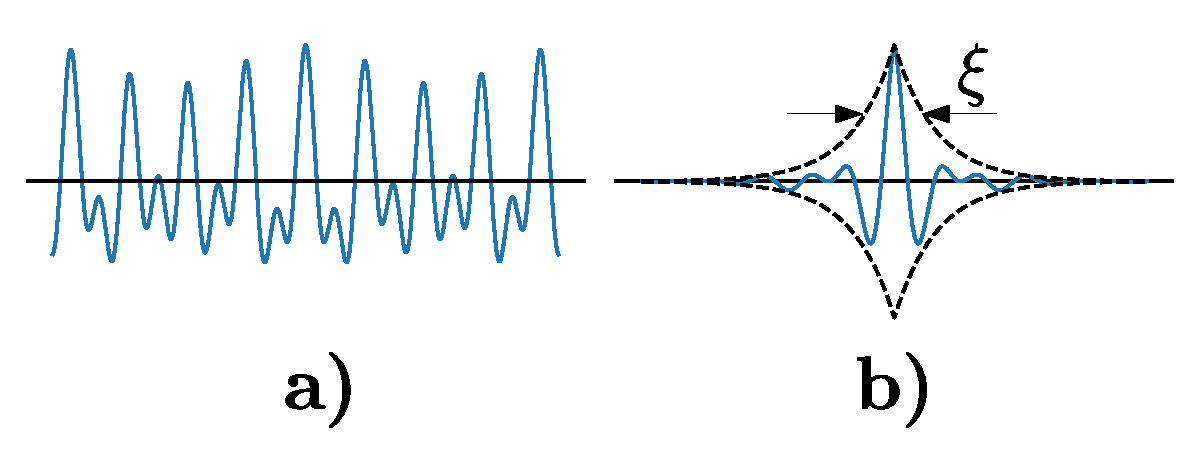
\includegraphics[width=1\textwidth]{diff_loc_ext_mod.pdf}}
\caption{ The Anderson theory of localization predicts that random potentials can localize quantum-mechanical states. An example of an extended state is shown in \textbf{a)}. A localized state whose envelope is exponentially decaying from some point in space is shown in \textbf{b)}.}
\label{fig:loc_ext_states} 
\end{figure}
\end{minipage}\\\\
\noindent 
 The existence of a critical energy or  the \emph{mobility edge} \cite{Mott_transitions} is now known to mark a disorder-driven phase transition between a metal and an insulator. The question of existence or nonexistence of extended states in two dimensions has been a point of contention for many years. According to the scaling theory \cite{scaling}, which shall be addressed in this seminar, all states are localized in two dimensions much as in the one-dimensional case, provided that the system is infinite. In 1977, less than twenty years after his groundbreaking paper, Anderson has been awarded with the Nobel prize for his work in the field.   \\\\
\noindent At the beginning of the seminar, a theoretical overview of basic concepts of disordered systems is provided in Sec. \ref{sec:basic}. Different models of disorder are discussed in Sec. \ref{sec:disorder}. Criteria of localization and results of numerical simulations are presented in Sec. \ref{sec:criteria}. We conclude in Sec. \ref{sec:conc}.
%REMOVE: true and quantum in disorder-driven phase transition 
% IMPORTANT, CHANGE: some inconsistencies regarding the use of fermi level and fermi energy; 


% While translational symmetry of ideally ordered crystalline solids permits classification of their corresponding electronic wave functions as spatially extended Bloch waves, this need not be the case with actual systems in which disorder may exist in varying degree, ranging from the presence of a few impurities, vacancies and dislocations in an otherwise perfectly crystalline host 
%references for this chapter: Lee, Ramakrishnan; Mott, Davis 
\section{The basic concepts of the disordered quantum systems}
\label{sec:basic}
In this section, an overview of the basic concepts of disordered quantum systems is given. We start off by briefly considering the theory of conductivity before the onset of localization theory, showing that the preceeding theories provide false predictions on the behaviour of conductivity in disordered systems. Turning our attention to the localization theory itself, we proceed by outlining the role that interference phenomena play in the onset of localization. Due to its particular importance, an interference effect known as enhanced back-scattering is discussed more in detail. The findings of the scaling theory, which provides a rather qualitative, yet highly instructive insight into the complex physics of localization, are discussed next. The section concludes with an explanation of the concept of the mobility edge, or the critical energy which separates extended and localized states in three dimensional disordered systems. Intuitive arguments for its existence are provided. 
% \begin{minipage}[t]{0.57\textwidth} In this section, an overview of the basic concepts of disordered quantum systems is given. How different models of disorder can be constructed from the staring point of an ideal translationally invariant systems is discussed first. The Anderson model is described in more detail as it is most commonly used
% to describe compositionally disordered alloys and was also used in numerical simulations presented in the following chapters of this seminar. The phenomenon of Anderson localization is approached by first considering the limits of weak and strong disorder, in which characterization of one-electronic wavefunctions can be made on rather intuitive grounds. The more complex region of intermediate disorder and dimensionality-dependent critical phenomena, such as the disorder-driven quantum phase transition in three dimensions, are discussed within the framework of the scaling theory. To conclude the section, localization criteria used in numerical simulations to determine presence or absence of localized states are introduced. 
% \end{minipage}\hfill
% \begin{minipage}[t]{0.4\textwidth}
% \begin{figure}[H]
% \centering{
% 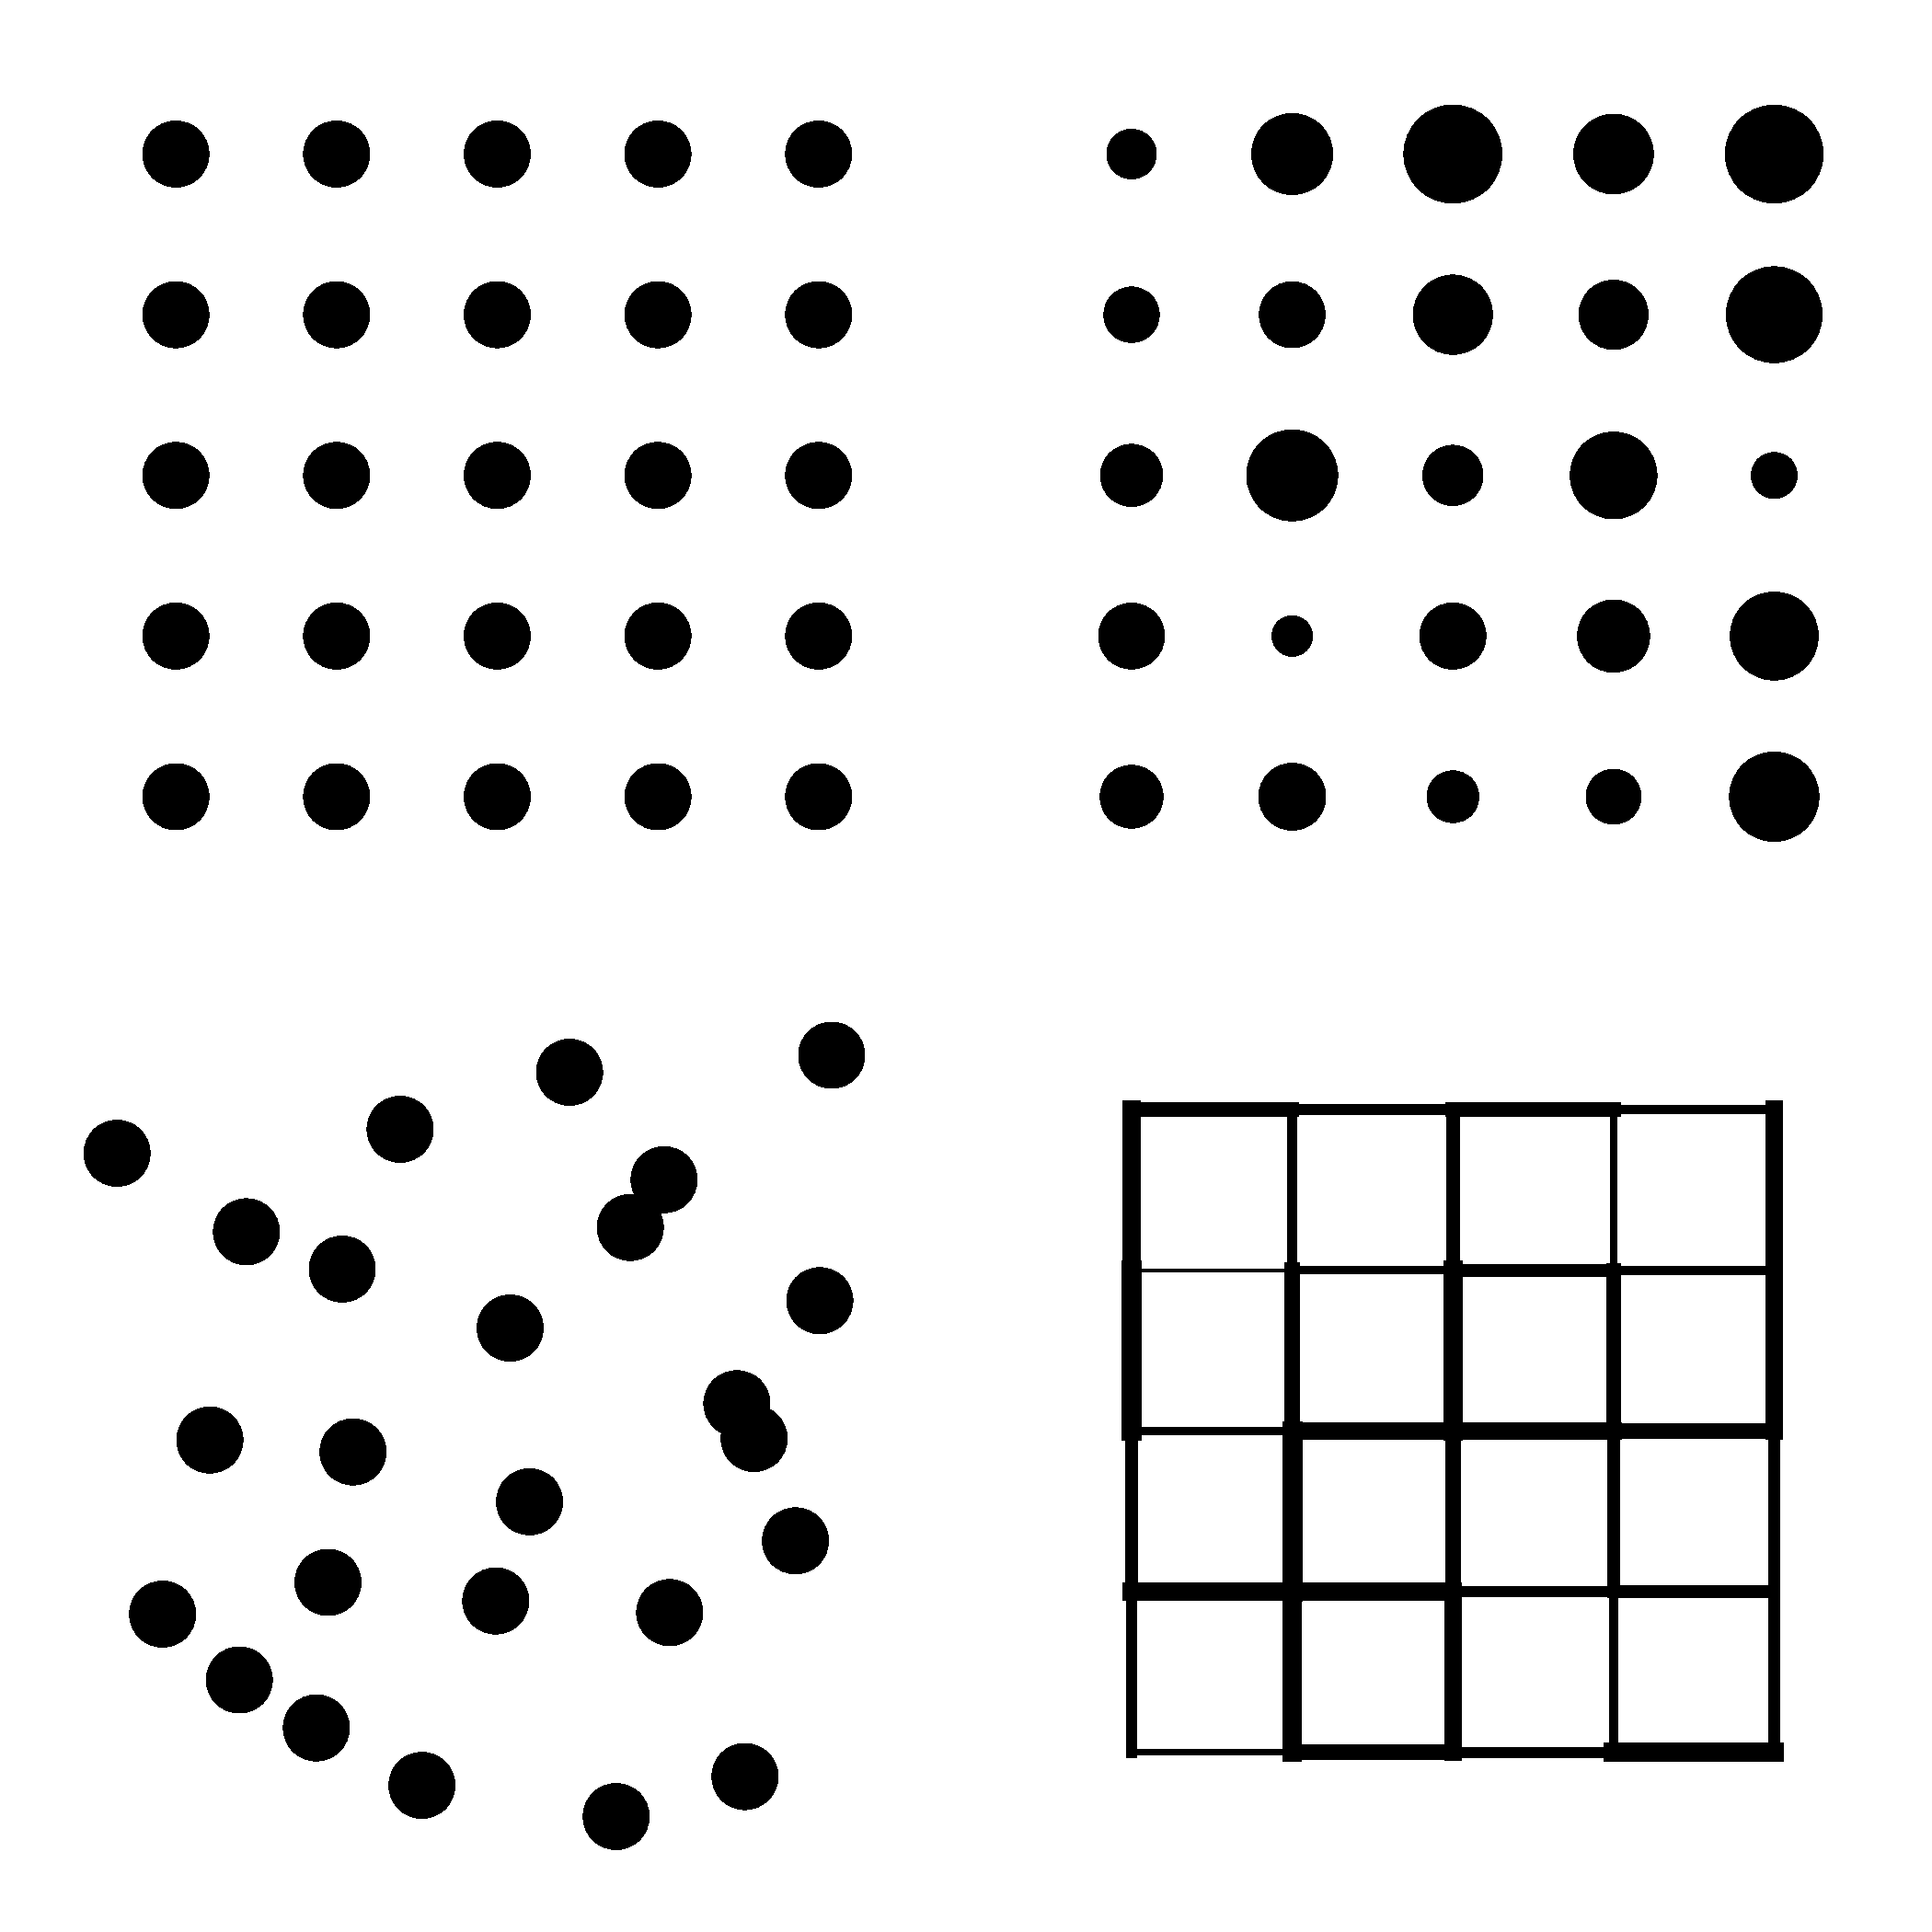
\includegraphics[width=0.7\textwidth]{disorder_scheme.pdf}}
% \caption{Schematics shown from left to right and top to bottom depict the following systems: an ideal crystal, a compositionally disordered system, structurally disordered system and a system with disorder in kinetic energy.  }
% \label{fig:disorder} 
% \end{figure}
% \end{minipage}
\subsection{Description of conductivity before and after the localization theory }
%to do: first: interference effects, quantum coherent back-scattering (weak localization), then strong localization; always reffer to the model structure and the tight-binding picture (see Mott, Davis) as this should be known from Condensed matter course; then proceed onto the introduction of the mobilty edge concept which is related to the band structure
The localization of quantum particles by a static random potential is an intriguing phenomenon of statistical physics. Prior to the advent of the Anderson theory of localization, the electronic conductance was usually described in terms of the quantum-mechanical revision of the classical Drude model. The latter assumes the electronic conductivity should be directly proportional to the mean-free path $l$, the average distance a particle travels before colliding with an impurity. Quantum-mechanically, wave packets propagating through a disordered medium will be scattered by the random potential on average after traveling a distance $l$. This would cause them to lose their well-defined momentum, however, the wave functions should remain extended throughout the system despite the scattering. Such propagation is diffusive on larger length scales and while increasing disorder should therefore lower the conductivity by lowering the mean-free path, the conductivity should remain finite for any finite disorder. This traditional description of conduction in disordered systems turns out to be incorrect as shown by Anderson in 1958. In case of a sufficiently strong disorder, particles in a system may become localized with their wave function's envelope decaying exponentially from some point $\mathbf{r}_0$ in space as $|\psi(\mathbf{r})| \sim \exp\left(|\mathbf{r} - \mathbf{r}_0 |/\xi \right)$, where $\xi$ is the \emph{localization length}. In that case, diffusive particle propagation is not only reduced, but can come to a complete halt - the particle becomes trapped and the conductivity vanishes \cite{self-consistent}. In order get some intuition of this rather striking result, it is instructive to consider multiple interference of wave components scattered by randomly placed scattering centers - localization is foremost an interference phenomenon.





% % \subsection{Conductivity before and after the localization theory }
% % %to do: first: interference effects, quantum coherent back-scattering (weak localization), then strong localization; always reffer to the model structure and the tight-binding picture (see Mott, Davis) as this should be known from Condensed matter course; then proceed onto the introduction of the mobilty edge concept which is related to the band structure
% % The localization of quantum particles by a static random potential is an intriguing phenomenon of statistical physics. Prior to the advent of the Anderson theory of localization, the electronic conductance was described in terms of the quantum-mechanical revision of the classical Drude model. The latter assummes the electronic conductivity should be directly proportional to the mean-free path $l$, the average distance a particle travels before colliding with an impurity. Quantum-mechanically, wave packets propagating through a disordered medium will be scattered by the random potential on average after traveling a distance $l$. This would cause them to lose their well-defined momentum, however, the wave functions should remain extended throughout the system despite the scattering. Such propagation is diffusive on larger length scales and while increasing disorder should therefore lower the conductivity by lowering the mean-free path, the conductivity should remain finite for any finite disorder. This traditional description of conduction in disordered systems turns out to be incorrect as shown by Anderson in 1958. In case of a sufficiently strong disorder, particles in a system may become localized with their wave function's envelope decaying exponentially from some point $\mathbf{r}_0$ in space as $|\psi(\mathbf{r})| \sim \exp\left(|\mathbf{r} - \mathbf{r}_0 |/\xi \right)$, where $\xi$ is the \emph{localization length}. In that case, diffusive particle propagation is not only reduced, but can come to a complete halt - the particle becomes trapped and the conductivity vanishes. In order to see how this rather striking result comes about, one needs to consider multiple interference of wave components scattered by randomly placed scattering centers - localization is foremost an interference phenomenon.
\subsection{Enhanced back-scattering }
\label{sec:enhanced}
The importance of quantum interference in the onset of Anderson localization can be most clearly recognized in the limit of weak disorder and consequent weak scattering. Starting with elementary wave mechanics, let us suppose an electron is propagating in a disordered medium from point $\mathbf{r}_0$ to point $\mathbf{r}_1$. To obtain the total probability of electron's arrival at $\mathbf{r}_1$, one needs to sum the complex-valued probability amplitudes of all paths between the two points and square the complex-valued end result. The final probability consists of a sum of squares of individual amplitudes - the classical, inchorent contribution - together with many cross-product, interference terms. In most cases, one can assume that the phases of interference terms are distributed randomly in a disordered medium and hence their sum vanishes on average. Such an omission of interference terms restores the traditional description of conductivity in disordered systems and is obviously not always justified.\\\\
\begin{minipage}[t]{0.58\textwidth}
\noindent  
    Let us consider the probability amplitude $A_1$ for a particle starting at $\mathbf{r}_0$ to move along some path $C_1$ and returning back to the starting point, and the probability amplitude $A_2$ to move along some other path $C_2$, as shown in Fig. \ref{fig:paths}. The return probability for the two possible returning paths will be 
    \begin{equation}
w=|A_1 + A_2|^2=w_\mathrm{cl} + w_\mathrm{int},
\end{equation}
with $w_\mathrm{cl}=|A_1|^2 + |A_2|^2$ and $w_\mathrm{int}=2\Re\left(A_1^*A_2\right)$ \cite{self-consistent}. For different returning paths $C_1$ and $C_2$, the interference terms of many such combinations average out, as discussed above. However, if $A_2=A_r$ is the amplitude for a time-reversed path $C_1$ and the system is time-reversal invariant, $A_1=A_r$, then the proper consideration of interference terms yields a twice larger return probability than in the classical case:
\end{minipage}\hfill
\begin{minipage}[t]{0.39\textwidth}
\begin{figure}[H]
\centering{
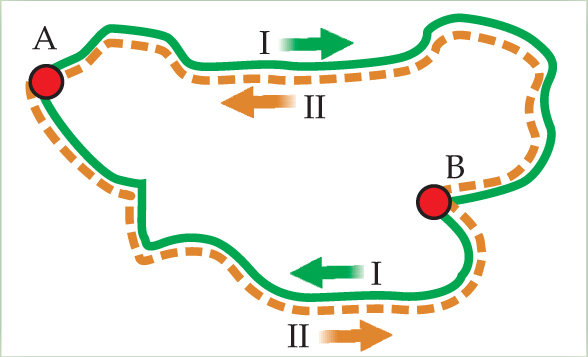
\includegraphics[width=0.9\textwidth]{interference.jpg}}
\caption{A schematic of a wave packet propagating from point A through point B back to A along path I and along its time-reverse II. Image was taken from \cite{50yearsof}.}
\label{fig:paths} 
\end{figure}
\end{minipage}
\noindent
\begin{equation}
w=4|A_1|^2=2w_\mathrm{cl}.
\end{equation}
In a scattering event, an outcome of an electron scattering back to its initial point is thus more likely than all other outcomes due to the constructive interference of a path with its time-reversed counterpart, which is often reffered to as the \emph{enhanced back-scattering}. The effect lowers the electron's transmission probability and hence also reduces conductivity. The effect is a precursor to localization.
% \noindent The above discussion is valid if the propagation is phase-coherent, meaning that the phase is not altered in a random manner during scattering events. This is the case if the scattering is static, e.g. the scatterers have no internal degrees of freedom, such as spins or phonons. In the zero-temperature limit, this effect alone leads to exponential localization of all states in one and two dimensions for any finite disorder. 
\subsection{The scaling theory}
In this section, we shed some light on the findings of the now widely-accepted \emph{scaling theory} of localization, which was put forth in 1979 by Abrahams, Anderson, Licciardello and Ramakrishnan \cite{scaling}. Though based on rather intuitive grounds, the theory provides a valuable insight into the role the dimensionality plays in localization phenomena. We note here that a complete and rigorous theoretical treatment of localization is still lacking. 
For one-dimensional systems, a rigorous proof by Mott and Twose \cite{Mott_Twose} exists, stating that all states are localized no matter how weak the disorder. In three dimensions, all states are localized above some critical disorder strength while both localized and extended states exist for subcritical disorder strengths. While no rigorous proof exists for the two-dimensional systems \cite{Kramer}, it appears that in the limit of an infinitely-sized system, all states localize for any nonzero disorder much as in the one-dimensional case. Finite-size systems, on the other hand, may display metallic properties.  
\\\\
\noindent Obviously, localization in disordered systems nontrivialy depends on the system's dimensionality. Despite its relative simplicity, the scaling theory succeeds in giving an elementary description of the dimensionality's role in localization phenomena. Within its framework, the Anderson localization is described in the language of critical phenomena of continuous (quantum) phase transitions. The latter occur at zero temperature and are driven by some parameter other than temperature. If disorder strength is considered as a driving parameter, this holds true in the case of Anderson localization as well. As any theory of phase transitions, the scaling theory predicts scaling laws for various quantities of interest among which we shall only briefly consider the conductance in this seminar. \\\\
The scaling theory of the conductance takes the conductance itself as its scaling variable. Before proceeding, we recall that in a three-dimensional ohmic conductor, the conductivity $\sigma$, an intensive property, and conductance $g$, an extensive property, are related by $g=\sigma \frac{S}{L}$. Here, $S$ is the conductor's cross-section area and $L$ its length. To describe the conductance $g(L)$ of a $d$-dimensional hypercube of the volume $L^d$, its logarithmic derivative $\beta$ is introduced:
\begin{equation}\label{eq:beta}
\beta=\frac{\mathrm{d}\log g}{\mathrm{d}\log L}.
\end{equation}
The theory assumes that $\beta$ depends only on $g$ itself, and not explicitly on energy, disorder or $L$. 
Its qualitative behaviour was obtained from the known asymptotic behaviour at large and small conductances
while an interpolation has been made in the intermediate region, assuming that $\beta$ is a continuous, monotonically increasing function. 
\\\\
\noindent
\begin{minipage}[t]{0.57\textwidth}
From Eq.\eqref{eq:beta} it is evident that the conductance $g$ increases with system size if $\beta>0$, which reflects metallic character. In the metallic region, the classical relation between the conductance and the conductivity holds,
\begin{equation}\label{eq:classical}
g(L)=\sigma \frac{L^{d-1}}{L}=\sigma L^{d-2}. 
\end{equation}
The relation for a three-dimensional ohmic resistor specified above is only a special case of the more general relation given by Eq. \eqref{eq:classical}, from which we obtain $\beta=d-2$ in the metallic region.
Consequently, $\beta$ is positive for three-dimensional conductors, zero for two-dimensional conductors and negative in one dimension. In the opposite limit, hence in the localized region, $g$ decays exponentially with system size, $g \propto \exp(-L)$, and so $\beta<0$.  Its precise functional dependence in this regime is given by 
\end{minipage}\hfill
\begin{minipage}[t]{0.42\textwidth}
\begin{figure}[H]
\centering{
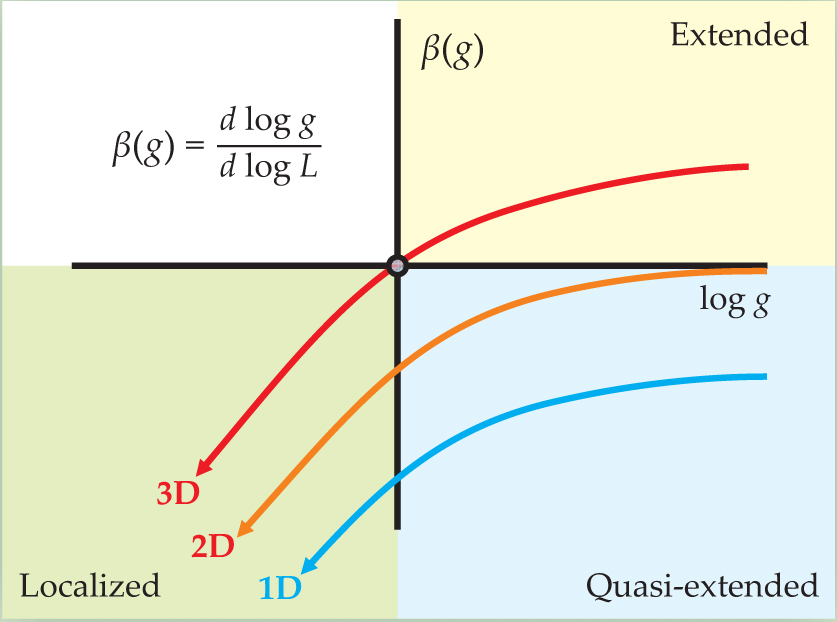
\includegraphics[width=0.8\textwidth]{beta_diagram.jpg}}
\caption{According to the scaling theory, a phase transition between a metal and an insulator can only occur in three-dimensional systems since the conductance always decreases in lower dimensional systems. Image was taken from \cite{50yearsof}.}
\label{fig:scalingtheory} 
\end{figure}
\end{minipage}\\\\
\noindent

% If $\beta<0$, on the other hand, $g(L)$ decreases with $L$ and eventually terminates in the localized region, where conductance is expected to decay exponentially, $g \propto \exp(-L)$. For $\beta$ in this region, we obtain
$$
\beta=\frac{\mathrm{d}\log g}{\mathrm{d}L}\frac{\mathrm{d}L}{\mathrm{d}\log L}=\log g
$$
The transition between an insulator and a metal occurs at the critical point $\beta(g_c)=0$.  This can only happen in three dimensions where $\beta$ can assume both negative  
and positive values while conductance always decreases with system size in lower dimensional systems and so the critical point is never reached.
\subsection{Existence of the mobility edge}
\label{sec:mob}
\begin{minipage}[t]{0.5\textwidth} 
In three dimensions, as shown by Anderson \cite{Anderson}, localization of all states only occurs if disorder is sufficiently strong. For weaker values of disorder, both localized and extended states exist in the system. For reasons that will not be discussed in this seminar, extended and localized states cannot coexist at the same energies, therefore there must be some critical, disorder-dependent energy $E_c$ separating them. Localized states cannot contribute to electron transport even if they emerge at the Fermi energy, while extended states do contribute to transport. For this reason, the critical energy $E_c$ is reffered to as the \emph{mobility edge}, a term coined by Mott who also introduced the physical concept \cite{Mott_transitions}. 
We will reffer back to the concept of the mobility edge in the subsequent sections once particular models of disorder and their numerical implementations are discussed. 

 % or the \emph{mobility edge}, is the critical energy determining whether a state is localized or not. To provide at least a qualitative justification for the existence of a mobility edge, let us now examine the tight-binding Hamiltonian given by Eq. \eqref{eq:anderson} in more detail. In lattice systems, a tight-binding Hamiltonian is an ideal array of equal potential wells, as shown in \textbf{a)} in Fig. \ref{fig:band_structure}. Energies of such a system are obtained by diagonalizing the Hamiltonian at $W=0$ using the Fourier transform. The dispersion relation for a system with a simple cubic unit cell of length $a$ is given by
% \begin{equation}\label{eq:dispersion_crystal}
% E_\textbf{k}=-2V\left(\cos(k_x a) +\cos(k_y a) +\cos(k_z a)\right).
% \end{equation}
\end{minipage}\hfill
\begin{minipage}[t]{0.45\textwidth} 
\begin{figure}[H]
\centering{
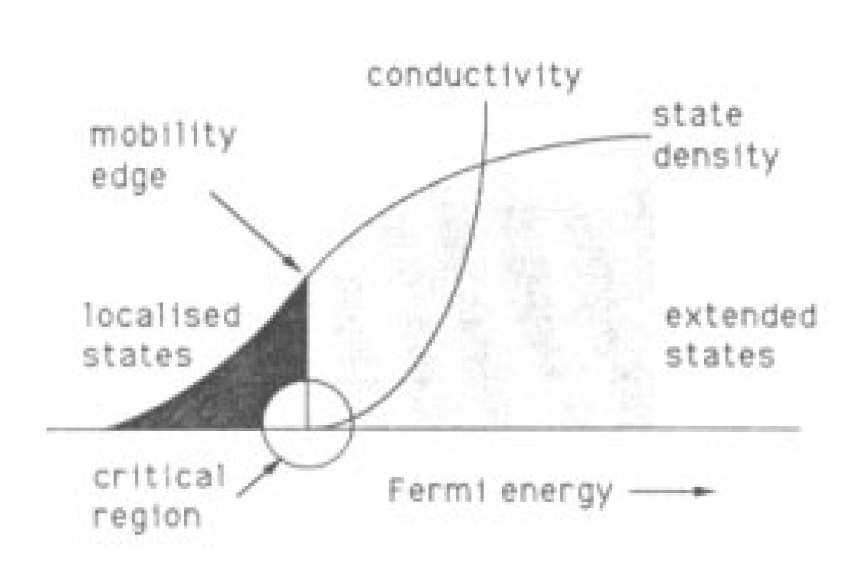
\includegraphics[width=1\textwidth]{mob_concept.png}}
\caption{A schematic explaining the concept of a mobility edge. Electronic states below $E_c$ are localized while those above it are extended. The system is insulating at $T=0$ if the Fermi energy lies in the region of the localized states. Image was taken from \cite{Kramer}.  }
\label{fig:band_structure} 
\end{figure}
\end{minipage}\\\\
\section{Models of disorder }
\label{sec:disorder}
% NOTE:MAKE A DISTINCTION BETWEEN TYPES OF DISORDER - amplitude and concentration of defects
In the previous sections, the most general properties and principles pertaining to the disordered quantum systems have been listed. In this section, we take a closer look at how specific models of disorder can be constructed. We proceed by taking the ideal crystalline structure as a staring point and discuss various ways of introducing disorder to such a system. The Anderson model is discussed in more detail as the most commonly used model of disorder which was also used in our numerical calculations. \\\\
\noindent
\subsection{Generic models of disorder}
In ideally ordered crystalline systems of non-interacting particles, characterization of their properties is made comparatively simple by their translational symmetry. One-electron wave functions are of the Bloch type and thus electrons are itinerant and can move in an unrestricted manner throughout such systems. In most actual systems, however, at least some degree of symmetry-breaking disorder is present, which can change the system's properties considerably. For systems with a low concentration of defects, on can still use the concepts of translationally invariant systems as a starting point in providing a description of the distorted systems. On the other hand, when the concentration of the distortions is large, one needs to abandon the translational symmetry altogether and new methods need to be developed. \\\\
\noindent  
\begin{minipage}[t]{0.6\textwidth}
\noindent As shown in Fig. \ref{fig:disorder}, various models of disorder can be constructed by somehow distorting the ideal crystal structure. By relaxing the lattice structure, models of \emph{structurally} disordered systems, such as amorphous semiconductors, can be obtained. In the continuous space representation, the one-particle Hamiltonian of such a system is given by
\begin{equation}\label{eq:amorphous_hamiltonian}
H=\frac{\hat{p}^2}{2m} + \sum\limits_{j=1}^N V_j(\mathbf{r}-\mathbf{R}_j),  
\end{equation}
where $\hat{p}$ is the momentum operator, $m$ particle's effective mass and $V_j$ the potential energy of an atom at the site $\mathbf{R}_j$. Disorder is introduced by taking both the potential energies and the site positions $\mathbf{R_j}$ at random and assuming some normalized probability density distribution function for the atomic potentials. In the case when a simple uniform probability distribution function is used, the model is used extensively in the theory of \emph{enhanced back-scattering}, which was addressed in Sec. \ref{sec:enhanced}.
\end{minipage}\hfill
\begin{minipage}[t]{0.38\textwidth}
\begin{figure}[H]
\centering{
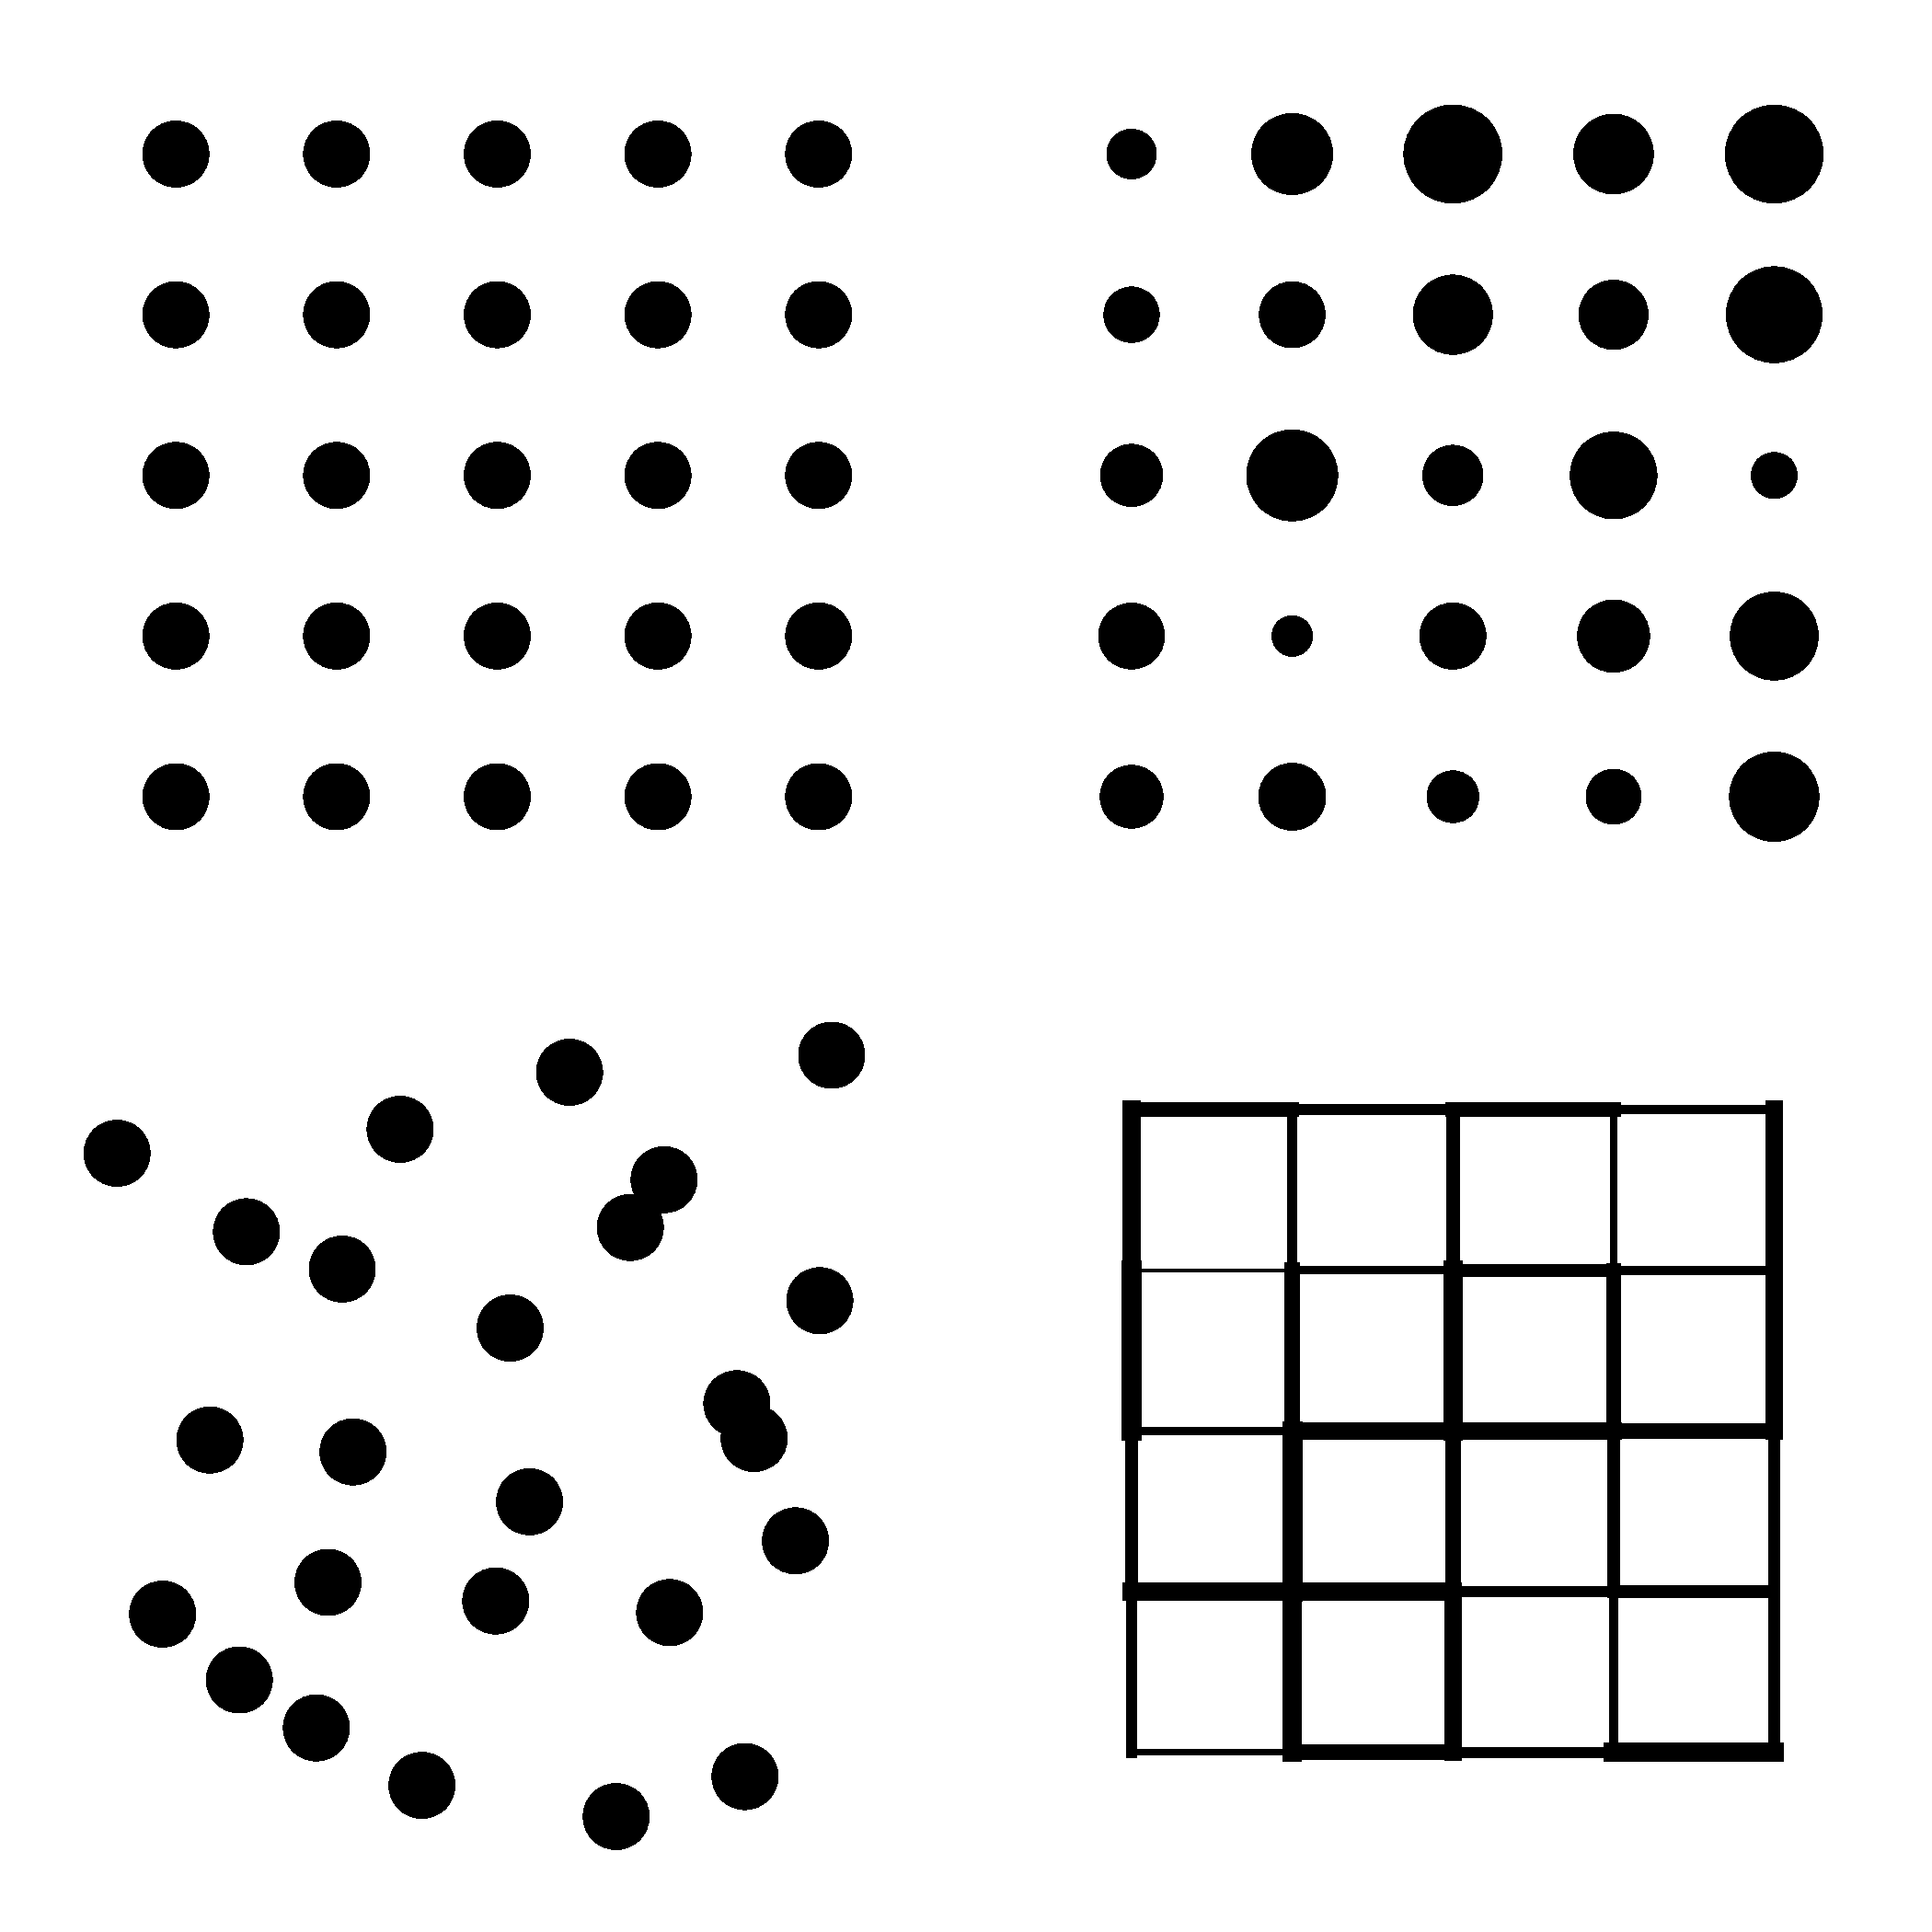
\includegraphics[width=0.7\textwidth]{disorder_scheme.pdf}}
\caption{Schematics shown from left to right and top to bottom depict the following systems: an ideal crystal, a compositionally disordered system, structurally disordered system and a system with disorder in kinetic energy.  }
\label{fig:disorder} 
\end{figure}
\end{minipage} \\\\
\noindent A different model is used in the studies of \emph{compositionaly} disordered solids, which are also the subject of this seminar's numerical calculations. Such systems are most often described by the following tight-binding Hamiltonian on a lattice:
% MAKE A DISTINCTION WITH THE PREVIOUS EQUATION
\begin{equation}\label{eq:compositional}
H=\sum\limits_{j\nu}\varepsilon_{j\nu} c^\dagger_{j\nu}c_{j\nu} + \sum\limits_{j\nu,k\mu} V_{j\nu, k\mu}c^\dagger_{j\nu}c_{k\mu}.
\end{equation}
% Here, $c^\dagger_{j,\nu}, c_{j,\nu}$ are fermionic creation and annihilation operators for a lattice site $j$ and state $\nu$. Labelled with $\varepsilon_{j\nu}$ in the diagonal part are the energies associated with states occupying particular lattice sites. The non-diagonal matrix elements $V_{j\nu, k\mu}$ correspond to quantum tunnelling transitions between states at different sites. Disorder is introduced by taking the site energies or hopping matrix elements (or both) at random and assumming some probability distribution for them. In our case, we consider the case of purely diagonal disorder with nearest-neighbour hoppint at a constant rate $V$, and with only one contributing one-electron orbital, $\nu=1$. According to the Anderson model, site energies $\varepsilon_j$ are drawn uniformly from the interval $[-W,W]$ according to the probability density function $p(\varepsilon_j)=\frac{1}{2W}\Theta(W-|\varepsilon_j|)$. Our model Hamiltonian thus has the form 
% \begin{equation}\label{eq:anderson}
% H=\sum\limits_j \varepsilon_j c^\dagger_jc_j + V\sum\limits_{\text{n.n.}} c^\dagger_{i}c_j + \text{h.c.}
% % NOTE: WRITE CORRECTLY FOR NEAREST NEIGHBOUR INTERACTIONS IN ALL DIMENSIONS!!!
% \end{equation}
\begin{minipage}[t]{0.5\textwidth} 
Here, $c^\dagger_{j,\nu}, c_{j,\nu}$ are fermionic creation and annihilation operators for a lattice site $j$ and state $\nu$. Labelled with $\varepsilon_{j\nu}$ in the diagonal part are the energies associated with states occupying particular lattice sites. The non-diagonal matrix elements $V_{j\nu, k\mu}$ correspond to quantum tunnelling transitions between states at different sites. Disorder is introduced by taking the site energies $\varepsilon_{j\nu}$ or hopping matrix elements $V_{j\nu, k\mu}$ (or both) at random and assumming some probability distribution for them. In contrast to the model given by Eq. \eqref{eq:amorphous_hamiltonian}, however, there is no structural disorder - lattice sites reside on well-defined positions in an ordered crystal lattice. \\\\
\noindent  
% In our case, we will be dealing with the \textbf{Anderson model} consider the case of purely diagonal disorder with nearest-neighbour hopping at a constant rate $V$, and with only one contributing one-electron orbital, $\nu=1$. In the Anderson model, site
\end{minipage}\hfill
\begin{minipage}[t]{0.45\textwidth}
\begin{figure}[H]
\centering{
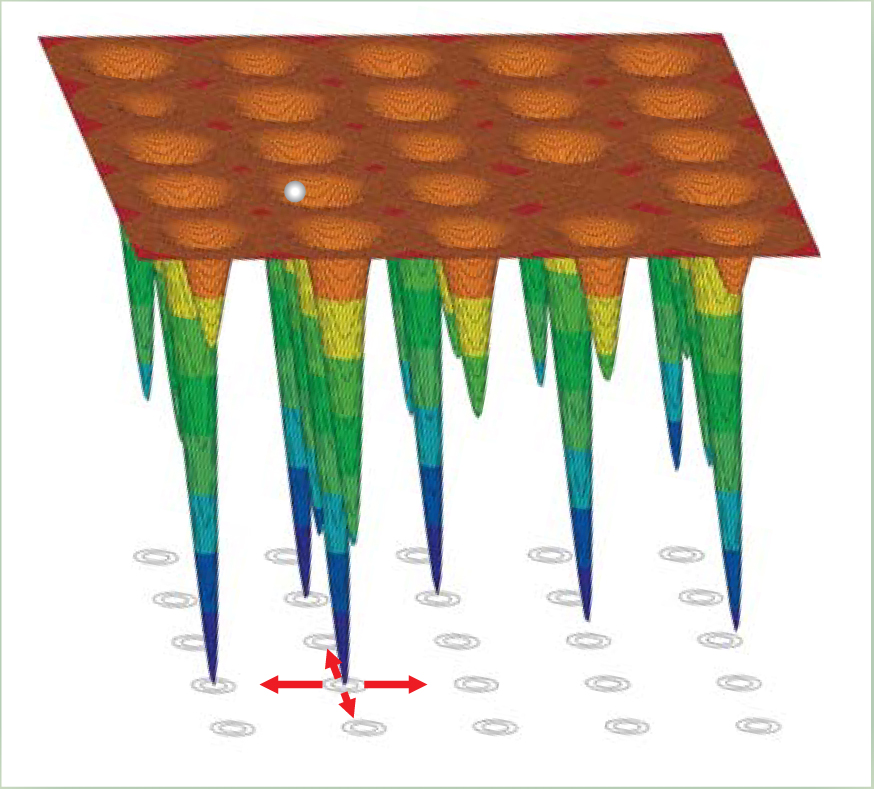
\includegraphics[width=0.5\textwidth]{hopping_picture_50years.jpg}}
\caption{A cartoon representing the physics of the Anderson model given by Eq. \eqref{eq:anderson}. A particle on an ordered lattice can hop to the nearest sites which have randomly varying site energies. Image was taken from \cite{50yearsof}.}
\label{fig:anderson_hopping} 
\end{figure}
\end{minipage}
\subsection{The Anderson model}
\label{sec:and}
\noindent The \textbf{Anderson model} \cite{Anderson} is obtained from the model in Eq. \eqref{eq:compositional} by assuming purely diagonal disorder with 
nearest-neighbour hopping at a constant rate $V$ and only one orbital, $\nu=1$. Site
energies  $\varepsilon_j$ are drawn uniformly from the interval $[-W,W]$ according to the probability density function 
\begin{equation}\label{eq:probability}
p(\varepsilon_j)=\frac{1}{2W}\Theta(W-|\varepsilon_j|),
\end{equation}
where $W$ is the disorder-strength parameter. Our model Hamiltonian thus has the form 
\begin{equation}\label{eq:anderson}
H=\sum\limits_j \varepsilon_j c^\dagger_jc_j + V\sum\limits_{\text{n.n.}} \left(c^\dagger_{i}c_j + \text{h.c.}\right)
\end{equation}
Unless explicitly specified, Hamiltonian given by Eq. \eqref{eq:anderson} is the one we will be referring to in the subsequent sections of the seminar. \\\\
\noindent 
\begin{minipage}[t]{0.56\textwidth} 
In lattice systems, a tight-binding Hamiltonian is an ideal array of equal potential wells, as shown in \textbf{a)} in Fig. \ref{fig:band_structure}. Energies of such a system are obtained by putting the Hamiltonian given by Eq. \eqref{eq:anderson} to the diagonal form using the Fourier transform at $W=0.$ The energies of such a system form a narrow band of width $2zV$, where $z$ is the coordination number \cite{Mott}. The Anderson Hamiltonian is obtained by changing the depth of each potential well by some random value $\varepsilon_j$ drawn from the distribution given by Eq. \eqref{eq:probability}. As shown schematically in \textbf{b)} in Fig. \ref{fig:band_structure}, introduction of disorder broadens the band while the density of states in a disordered system displays no singularities characteristic of the systems with long-range order. An argument due to Lifshitz, as presented in Sec. 4.2 of Ref \cite{Kramer}, states that the tails of the density-of-states distribution fall off exponentially, which is why they are often reffered to as the Lifshitz tails. \\\\
\noindent In the limit of very strong disorder, where the magnitude of the disorder parameter $W$ is estimated with respect to the hopping rate $V$, we can assume that the potential term in Eq. \eqref{eq:anderson} strongly prevails over the hopping term and thus localization of states is preffered. Using perturbation arguments, the Hamiltonian's eigenfunctions can be described as bound states or localized orbitals bound by deep fluctuations in the random potential. Since energies of such one-electron states are to a large extent determined by the depths of random potential wells, states with a significant spatial overlap differ considerably in energy. States with similar energies, on the other hand, are usually spatially distant and thus overlap negligibly. Failing to hybridize,  the states remain localized in strong disorder. \\\\
\noindent For intermediate disorder, both extended and localized states exist in a three-dimensional system, as established in Sec. \ref{sec:mob}. In the absence of disorder, the eigenstates of the Anderson Hamiltonian are extended wave functions of the Bloch type. Setting $W$ to a small  
\end{minipage}\hfill
\begin{minipage}[t]{0.42\textwidth} 
\begin{figure}[H]
\centering{
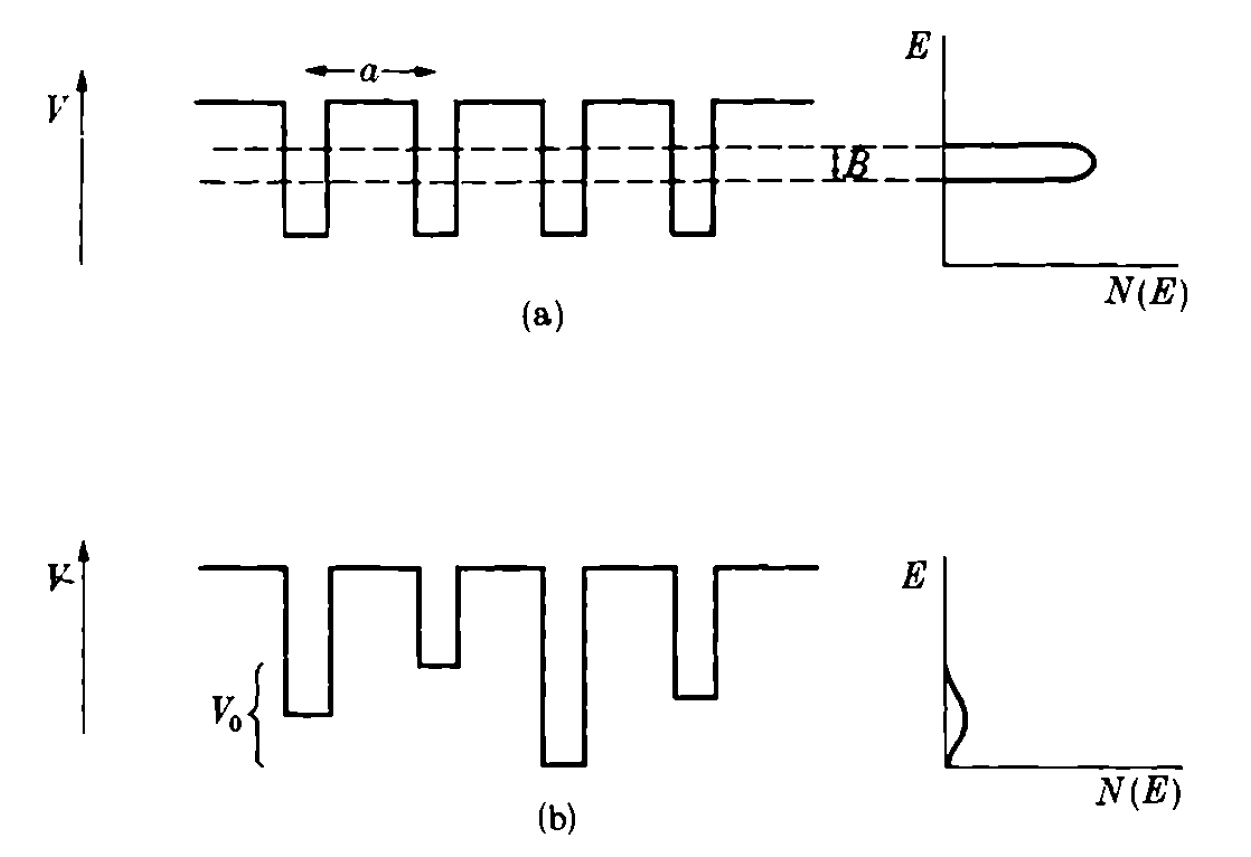
\includegraphics[width=1\textwidth]{bands.png}}
\caption{a) Potential wells in the tight-binding approximation in an ideal crystalline lattice. b) Potential wells for the Anderson lattice with randomly varying potential strengths. Schematics of the densities of states in three dimensions are shown on the right. Introduction of disorder broadens the band and smooths out singularities in the density of states. Image was taken from \cite{Mott}.  }
\label{fig:band_structure} 
\end{figure}
\begin{figure}[H]
\centering{
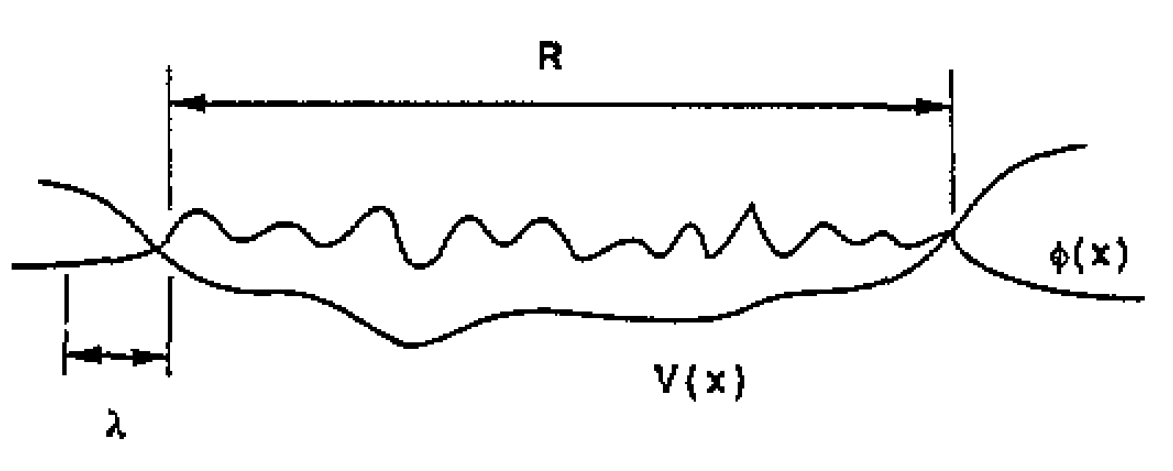
\includegraphics[width=0.95\textwidth]{accidental_wells.png}}
\caption{In a compositionally disordered medium, the site potential energy varies randomly from site to site. Accidental potential wells can be formed, outside of which wave functions are not of oscillating, but of exponentially decaying character instead. Image was taken from \cite{Kramer}.}
\label{fig:accidental_wells} 
\end{figure}
% \begin{figure}[H]
% \centering{
% 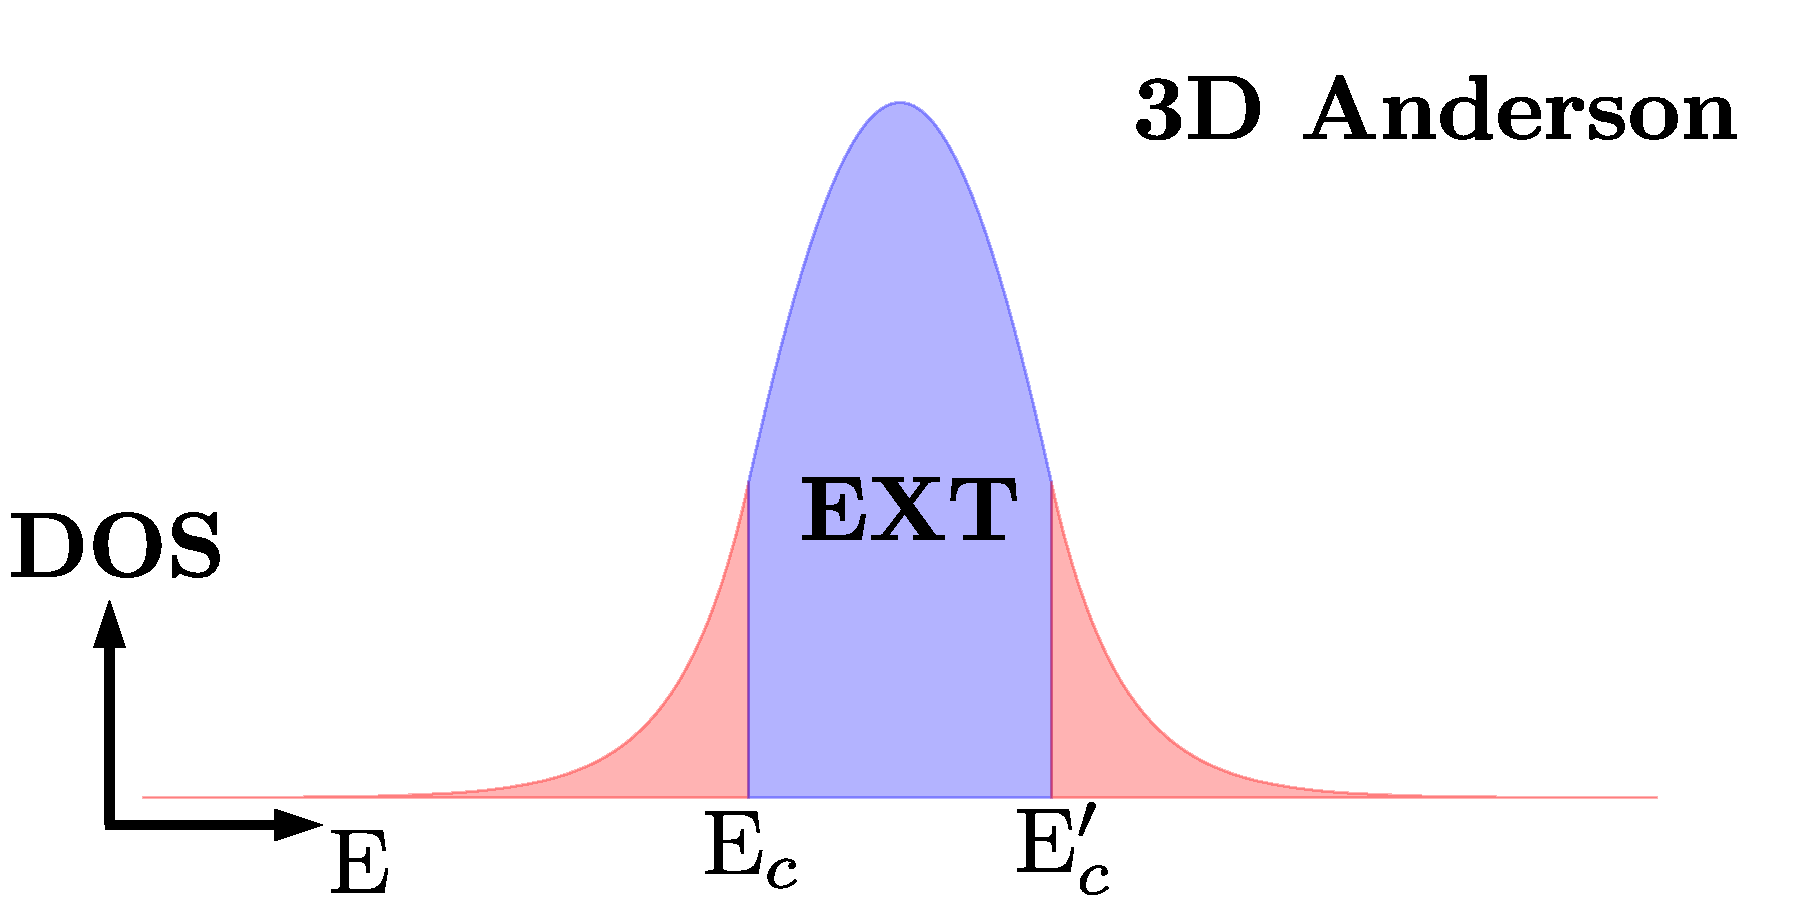
\includegraphics[width=0.95\textwidth]{mobility_edge_DOS_modified.pdf}}
% \caption{A schematic of a typical density of states (DOS) distribution with respect to energy for a three-dimensional Anderson model for some intermediate disorder $W<W_c$. States in the band tails (coloured red) are localized while those in the middle (coloured blue) are extended. }
% \label{fig:DOS} 
% \end{figure}
\end{minipage}\break
nonzero value introduces weak random potential fluctuations, which should only affect the states near the band extrema, while 
leaving those near the center of the band mostly unaffected. This view can be related with the formation of \emph{accidental} potential wells such as the one shown in Fig. \ref{fig:accidental_wells}. Weak potential fluctuations can only form shallow potential wells which in turn might only localize the low energy eigenstates. Increasing the disorder strenght further, even states higher in energy might become localized. Due to the particle-hole symmetry of the Anderson Hamiltonian, there are in fact two mobility edges, $E_c$ and $E'_c$, symmetric with respect to the center of the band, as shown in Fig. \ref{fig:DOS}. The two values are aproaching the band center upon increasing $W$ - full localization occurs once they merge at some critical value of the disorder parameter $W_c$.
\begin{figure}[H]
\floatbox[{\capbeside\thisfloatsetup{capbesideposition={left,center},capbesidewidth=6cm}}]{figure}[\FBwidth]
{\caption{A schematic of a typical density of states (DOS) distribution with respect to energy for a three-dimensional Anderson model for some intermediate disorder $W<W_c$. States in the band tails (coloured red) are localized while those in the middle (coloured blue) are extended, which is denoted by \textbf{EXT} in the figure. $E_c$ and $E'_c$ denote the mobility edges.  }\label{fig:DOS}}
{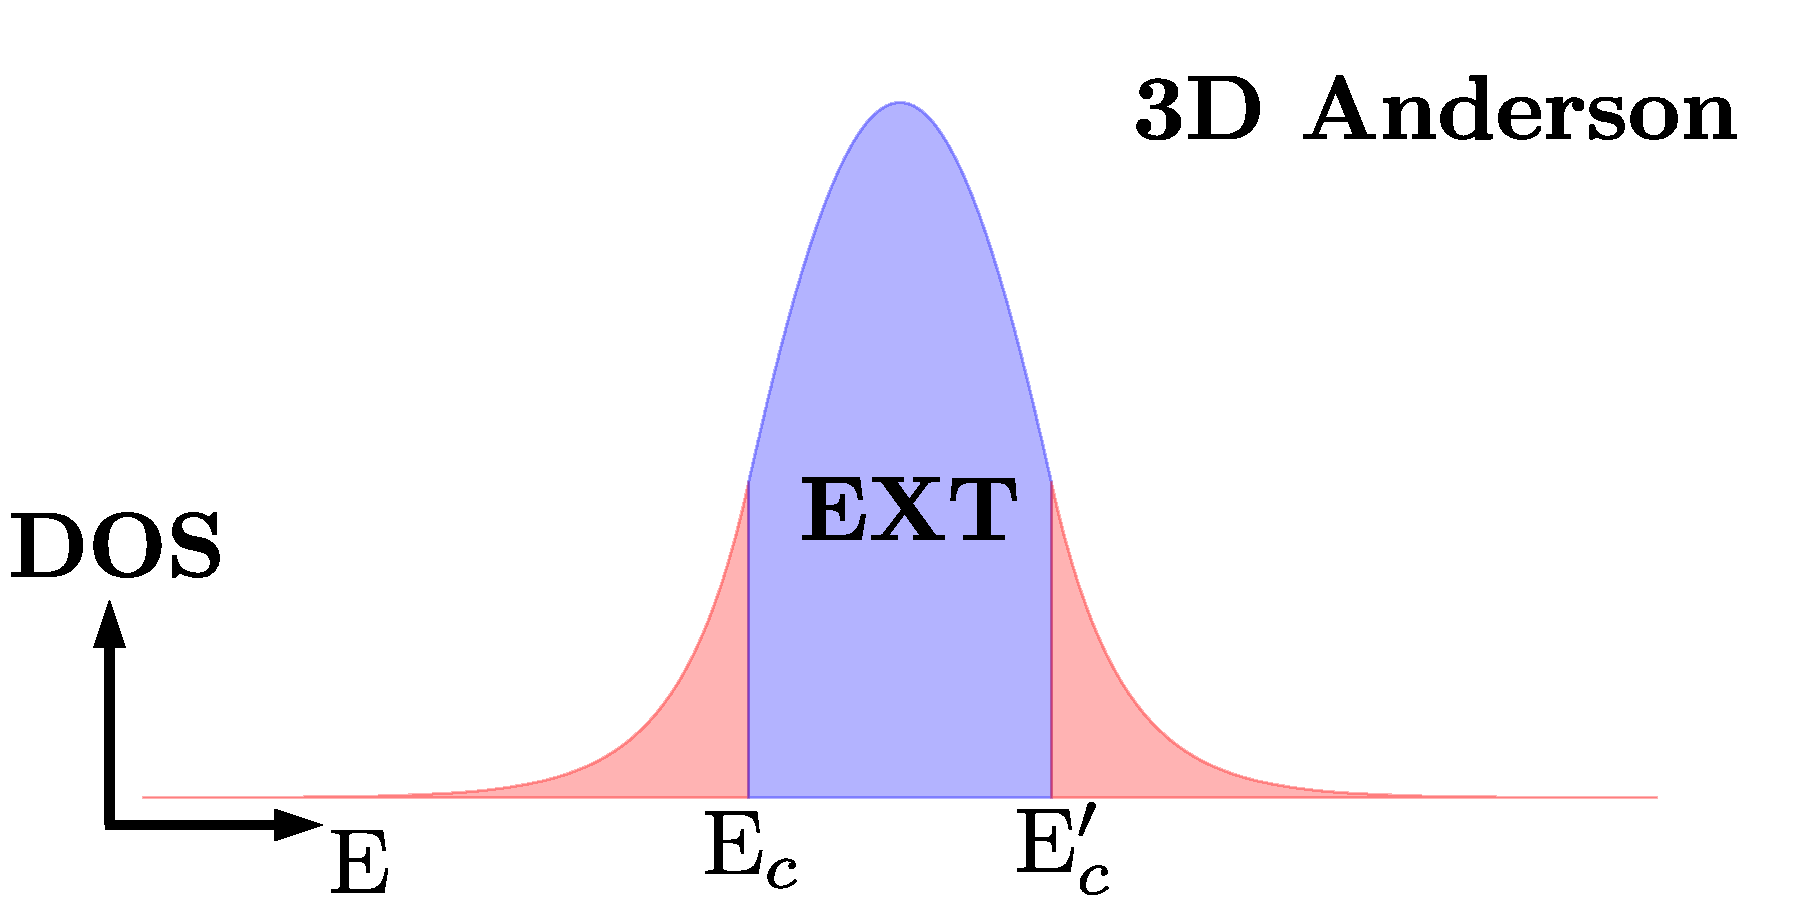
\includegraphics[width=0.45\textwidth]{mobility_edge_DOS_modified.pdf}}
\end{figure} 
\subsection{Numerical implementation of the Anderson model}
\label{sec:num}
In his Nobel lecture in 1977 \cite{and_nobel}, P.W. Anderson famously asserted that  ``one has to resort to the indignity of numerical simulations to settle even the simplest questions about localization.'' More than 40 years later, this is still very much the case - in order to test the theoretical considerations of the preceeding sections, we have resorted to performing numerical simulations in \url{Python2} programming language. The Anderson Hamiltonian with imposed open boundary conditions has been numerically implemented in one, two and three dimensions.  Calculations were run on the compute nodes of the F-1 cluster at the Jožef Stefan Institute, utilizing the \url{intelpython} distribution of \url{Intel}'s optimized numerical libraries. Exact diagonalization of the Hamiltonian and time-evolution of an initial wavefunction have been performed, implementation-specific details of which are discussed below. Results are presented in the next section.\\\\
\noindent Random distributions of the Hamiltonian's diagonal elements were simulated using the function \url{random.uniform(low=-W,high=W)} from the \url{numPy} library. For a given disorder strength $W$, calculations had to be performed for sufficiently many different realizations of the random potential, since quantum-mechanical observables in a system with random disorder are only physically relevant if they are averaged across different realizations of the disorder. Between 30 and 200 such realizations have usually been made, where the larger number was typically needed for higher disorder strengths. The hopping rate $V$ has been set to the value of 1 in all of our calculations.\\\\
\noindent Exact full diagonalization studies have been performed using the \url{linalg.eigh()} function from the \url{numPy} library which is used for diagonalizing hermitian matrices. Analysis of the finite-size effects has also been made by performing diagonalization calculations on different system sizes for a given disorder strength. Once different disorder realizations, different system sizes and different disorder strenghts are combined, it quickly becomes obvious that the number of pending calculations can become overwhelmingly large. For this reason, we have limited our calculations to smaller maximum lattice sizes: 1000 sites in 1D, $(100\times100)$ sites in 2D and $(22\times22\times22)$ sites in 3D. \\\\
Time evolution studies have been performed by time evolving the initial wave function according to the propagation scheme
\begin{equation}\label{eq:propagation}
\ket{\psi, t+\mathrm{d}t}=\exp\left(-\mathrm{i}\hat{H}\dd t\right)\ket{\psi, t},
\end{equation}
where the time propagator in the above equation has been approximated by its Taylor expansion up to tenth order. To preserve the wave function's norm, renormalization has been made at each time step. Making use of the Hamiltonian's sparse structure, functions from the \url{SciPy.sparse} package have been used. Using a time-step length of $\dd t=0.1$, $N_\mathrm{iter}=10000$ iteration steps have been performed in all time-evolution studies presented in this seminar.   
 \section{Criteria for localization}
 \label{sec:criteria}
In this section, the criteria used to determine the presence of localized states in the system are presented together with the results of the numerical studies. We focus in particular on the two criteria widely used in the literature, namely the \emph{inverse participation ratio} and the \emph{absence of diffusion}. The main goal of this section is to provide the reader with an impression of how the actual numerical simulations of the Anderson localization look like, and which are the main difficulties faced when determining the precise values of the localization transition.
\subsection{The inverse participation ratio}
\noindent Whether a state is localized or extended can be determined by considering the second moment of the probability density or the inverse participation ratio as defined in Sec. 5.2 of Ref. \cite{Kramer}:
\begin{equation}\label{eq:inverse_part}
P^{-1}=\sum\limits_\mathbf{r} |\psi(\textbf{r})|^4, \hspace{5mm} \norm{\psi}=1.
\end{equation}
The inverse participation ratio is a measure of the portion of the space where the wavefunction differs markedly from zero and takes a value of $1$ for a wavefunction localized at a single site while its value is small for extended states. It also provides a measure for an average diameter $\tilde{R}$ of a state via $\tilde{R}=P^{1/d}$. One obtains $P=L^d$ for plane waves in which case $P$ equals the system volume. Divergence of $\tilde{R}$ in the $L\to\infty$ limit is considered as the representative behaviour of extended states. 
 In our numerical simulations, the studies of $P^{-1}$ have been performed by first exactly diagonalizing the Hamiltonian given by Eq. \eqref{eq:anderson} for a given realization of disorder:
\begin{equation}\label{eq:diagonalizacija}
\hat{H}\ket{\psi_\alpha} = E_\alpha\ket{\psi_\alpha}.
\end{equation}
Here, $E_\alpha$ and $\ket{\psi_\alpha}$ denote the Hamiltonian's eigenenergies and eigenstates, respectively. The inverse participation ratio $P^{-1}_\alpha$ of each of the eigenstates was then calculated according to Eq. \eqref{eq:inverse_part}, and the final results were obtained by averaging $P_\alpha^{-1}$ values over different disorder realizations. Finite-size analysis was done by repeating the above procedure for different system sizes and calculating the average spectral inverse participation ratio, defined as 
\begin{equation}\label{eq:P_ave}
\bar{P}=\frac{1}{N_\alpha}\sum\limits_\alpha^{N_\alpha} P_\alpha.
\end{equation}
Here, $N_\alpha$ is the number of eigenstates. $\bar{P}$ goes towards zero in the limit of an infinite system in the fully extended case while it should assume a finite value if localization occurs. Results of the numerical simulations in the 1D, 2D and 3D case are presented below. 
\begin{figure}[H]
\centering{
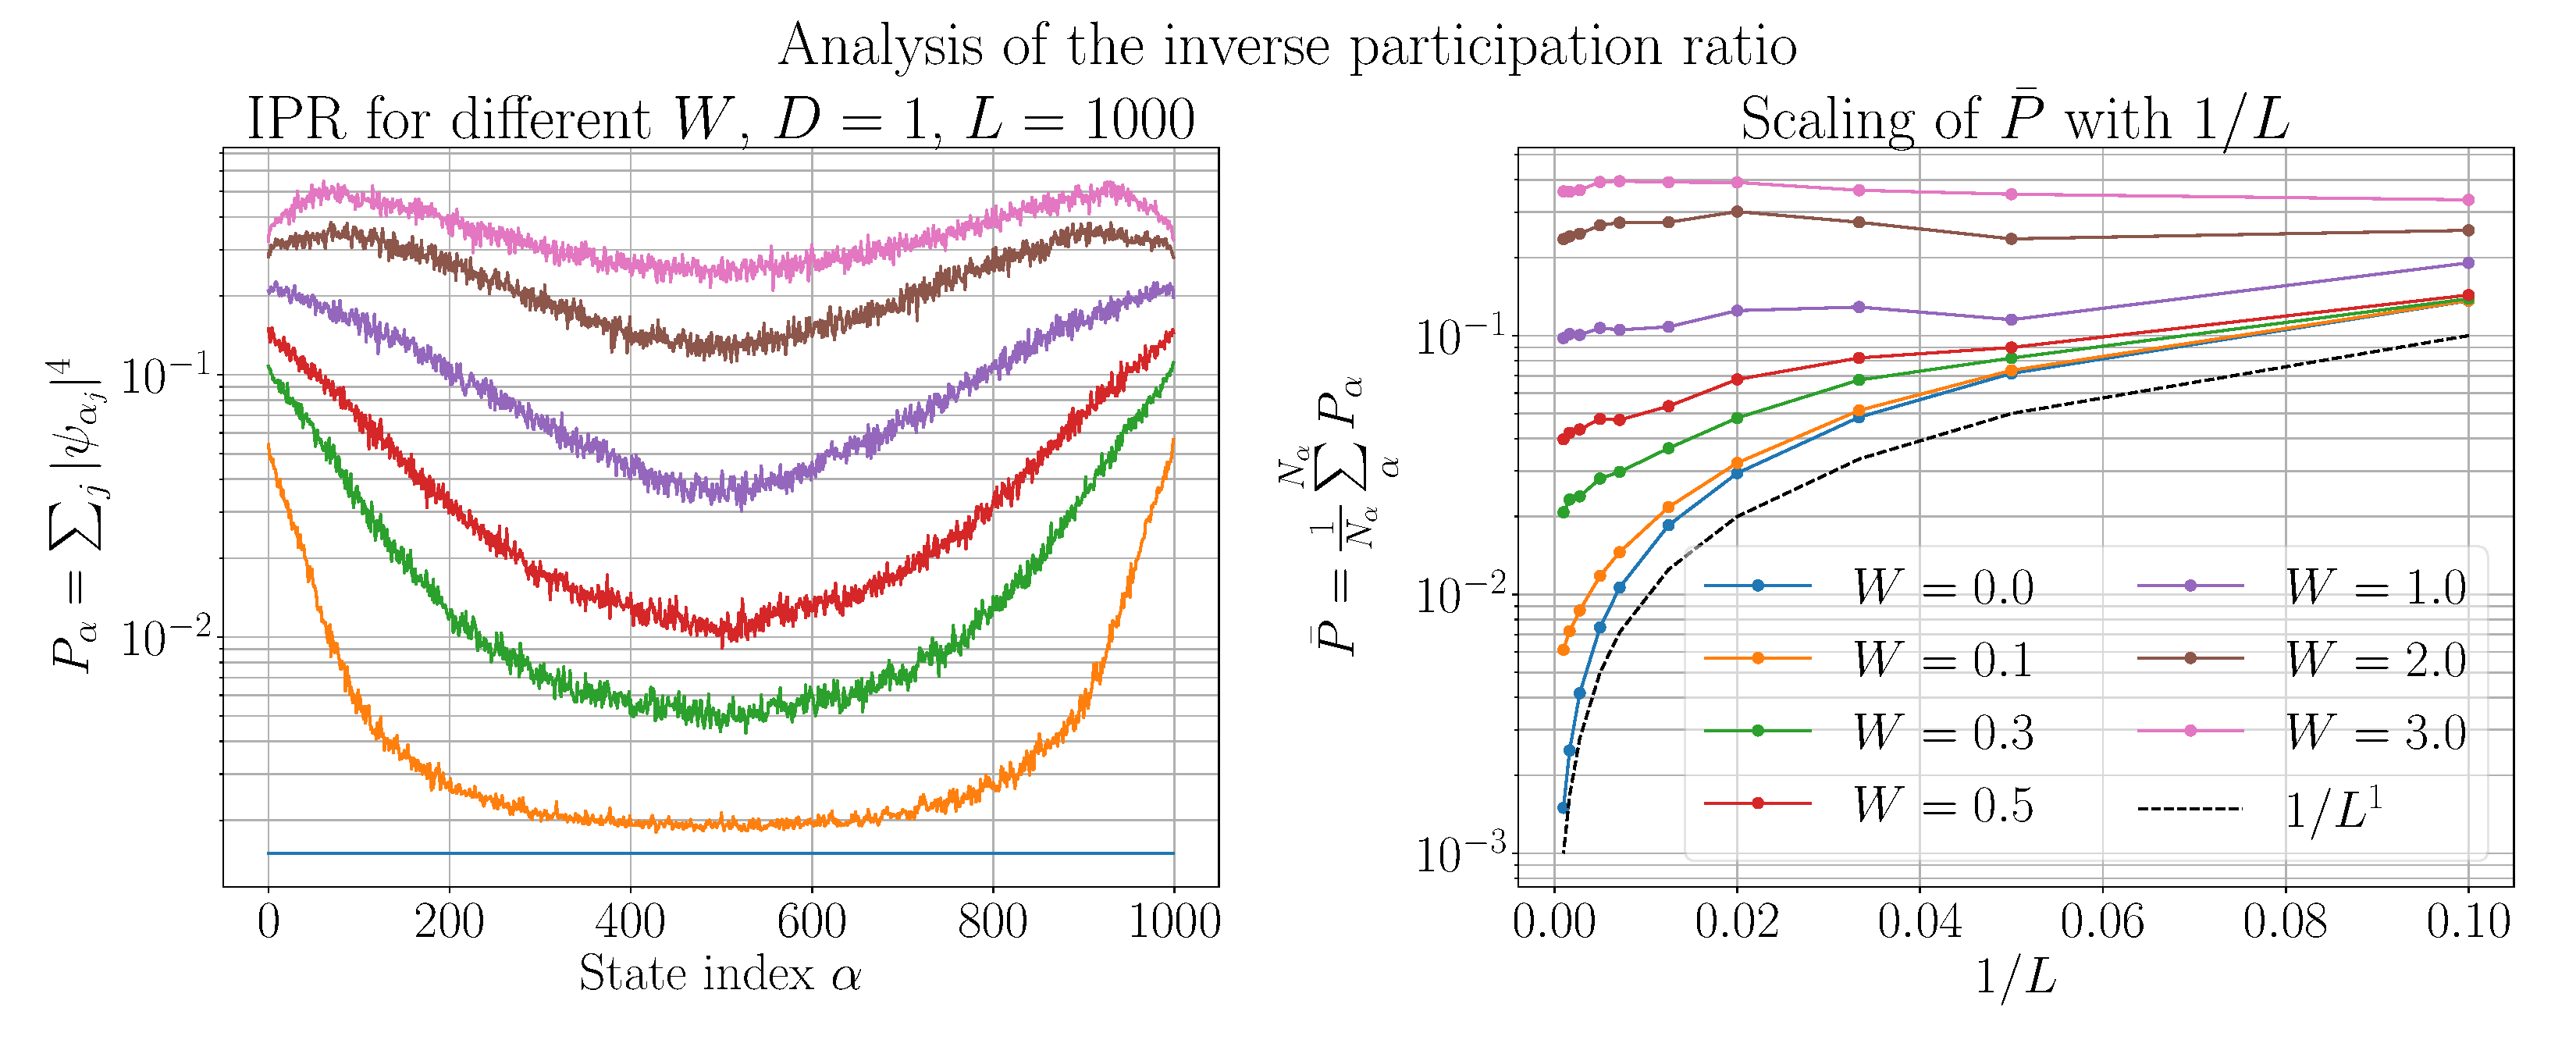
\includegraphics[width=1\textwidth]{1D_Anderson_localization_Seminar_scaling_analysis_D1_shape_1000_ipr_plots.pdf}}
\caption{Studies of the inverse participation ratio in the one-dimensional case. Left: values of $P^{-1}_\alpha$ with respect to the eigenstate index $\alpha$ for different realizations of disorder, calculated for a lattice with $L=1000$ sites. Greater $P^{-1}_\alpha$ values mean greater degree of localization where the $W=0.0$ curve corresponds to the extended case. In accordance with the theory discussed in \autoref{sec:and}, greater degree of localization is observed near both band edges and the curves appear symmetric with respect to the band center. In the $W=0.1$ case, the low $P^{-1}_\alpha$ values near the band center imply the states appear extended for a given system size, which is a finite-size effect. Right: finite-size scaling analysis of $\bar{P}$ given by Eq. \eqref{eq:P_ave} with respect to the inverse system size $1/L$. The results for small $L$ show that extended and localized regimes are hardly discernible in smaller systems while the difference becomes prominent once larger systems are considered.   }
\label{fig:1D_ipr} 
\end{figure}
\noindent
In the 1D case, as shown in the left graph in Fig. \ref{fig:1D_ipr}, finite size effects become prominent at small disorder strengths. For $W=0.1$, the $P_\alpha^{-1}$ values near the band center closely approach the ones for the case without disorder. Even though extended states should not exist for any finite disorder in lower-dimensional systems, the states might appear extended in a finite system if their localization length is comparable to the lattice size. The scaling analysis shown in the same figure reveals that systems with low disorder are hardly discernible from the ones with no disorder if calculations are performed on smaller lattices.\\\\ 
\begin{figure}[H]
\centering{
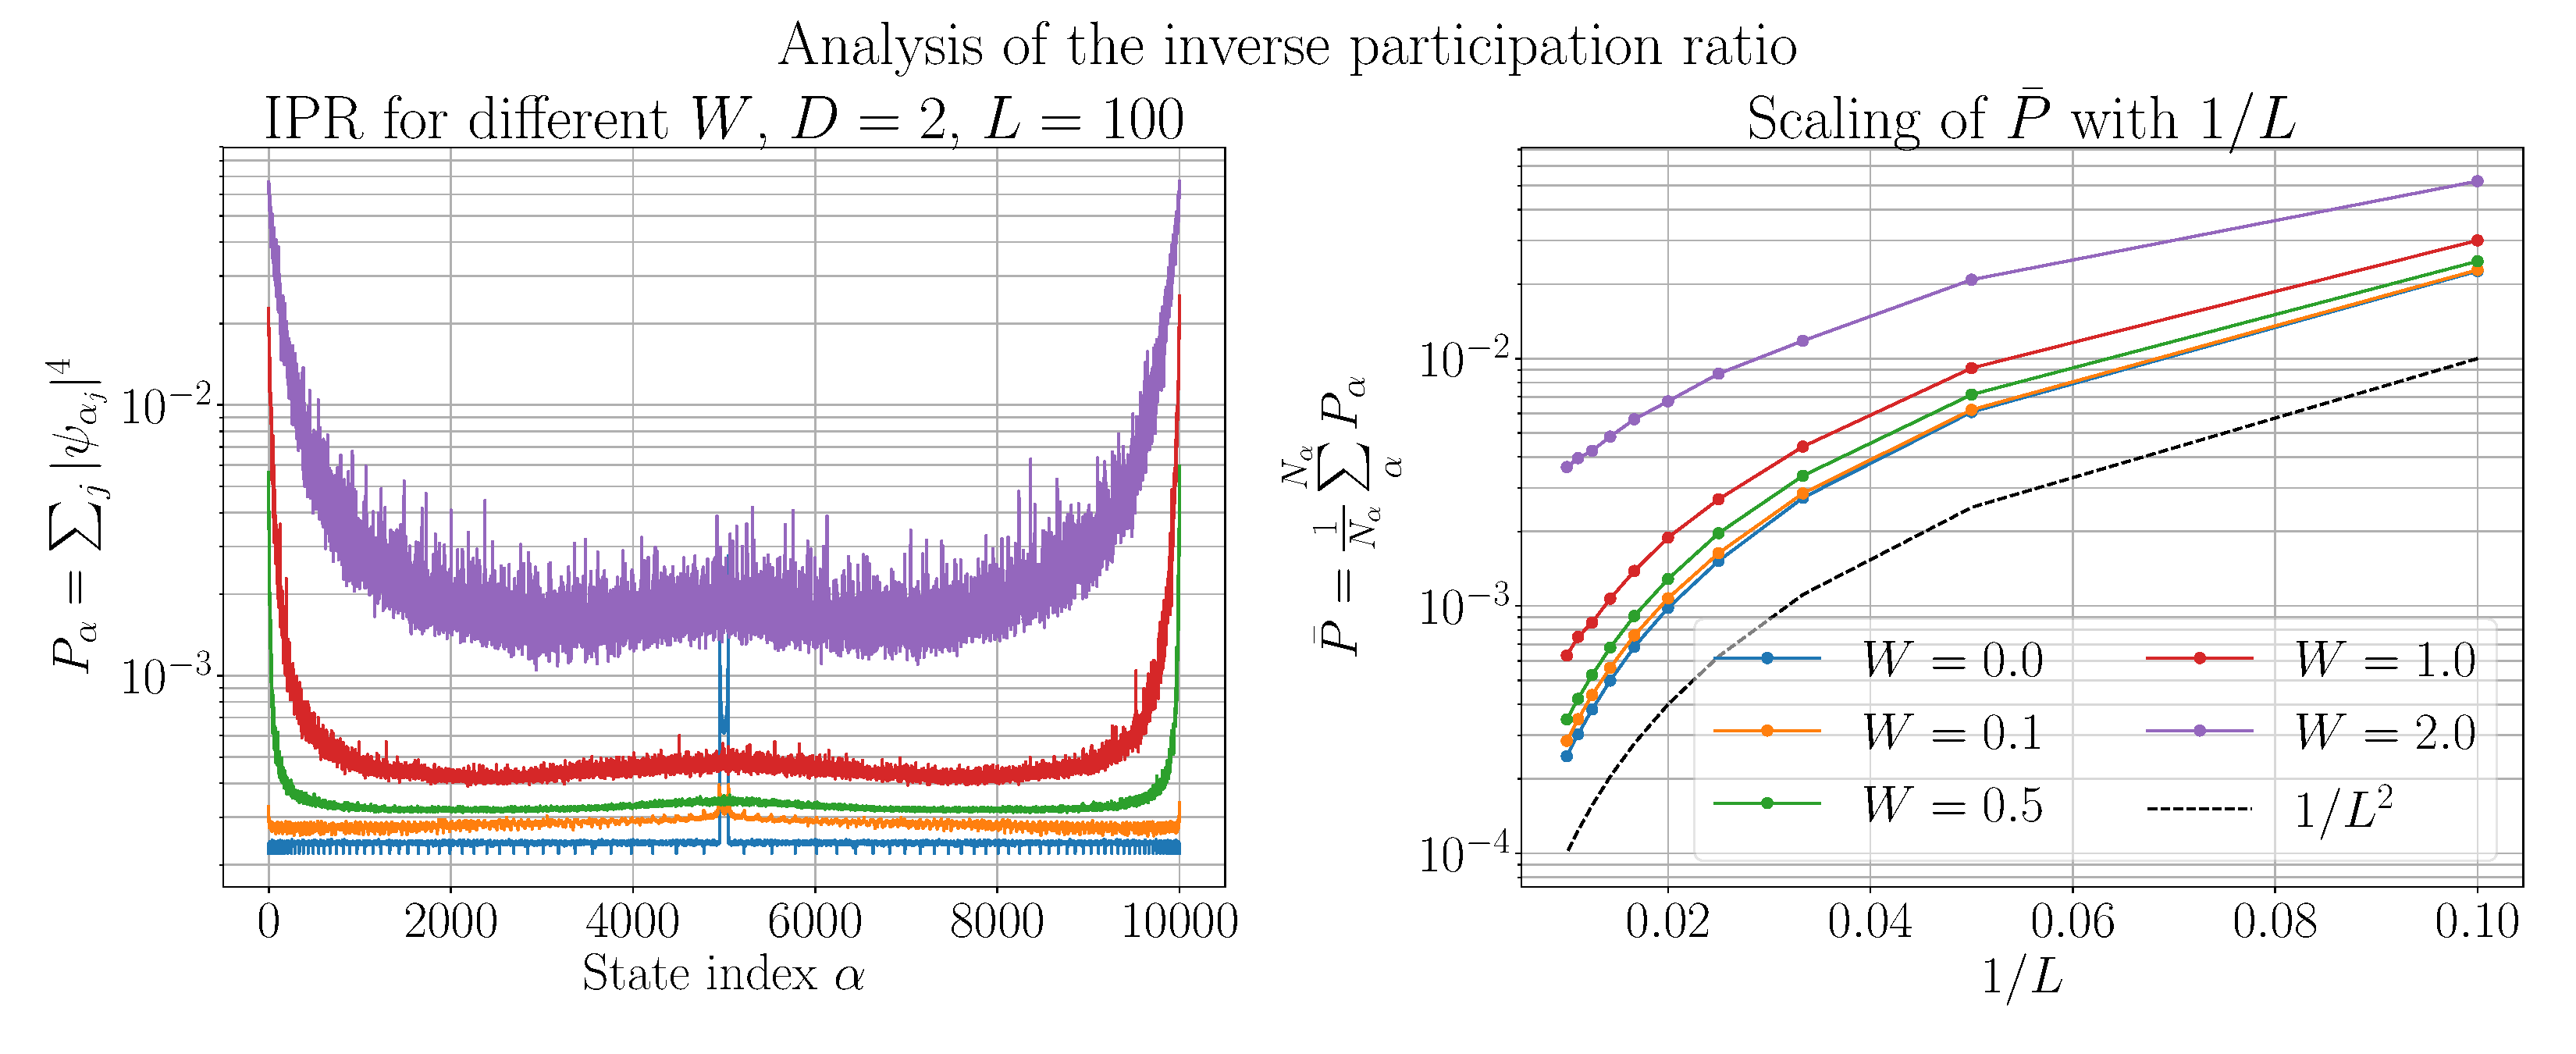
\includegraphics[width=1\textwidth]{2D_Anderson_localization_Seminar_scaling_analysis_D2_shape_100_100_ipr_plots.pdf}}
\caption{Studies of $P^{-1}_\alpha$ and $\bar{P}$ in 2D with averaging over 30 random disorder realizations. Full localization is evident in the $W=2.0$. Since the finite Hilbert space dimension equals the number of lattice sites, the maximum lattice size considered in the finite-scaling analysis equaled $(100\times100)$ sites due to the reasons given in Sec. \ref{sec:num}}
\label{fig:2D_ipr} 
\end{figure} 
\begin{figure}[H]
\floatbox[{\capbeside\thisfloatsetup{capbesideposition={left,center},capbesidewidth=6cm}}]{figure}[\FBwidth]
{\caption{IPR studies on a 3D lattice with $(22\times22\times22)$ sites with averaging over 50 disorder realizations. For $W=0.5$, only the states near the band extrema appear localized, while other states remain extended. Increasing disorder to $W=1.0$, we observe that only states near the band center remain extended, which corresponds to an increase in $E_c$ for an increase in disorder. Unexpected sharp peaks in the $W=0.1$ curve are due to the limitations of the numerical diagonalization routine used.}\label{fig:3D_ipr}}
{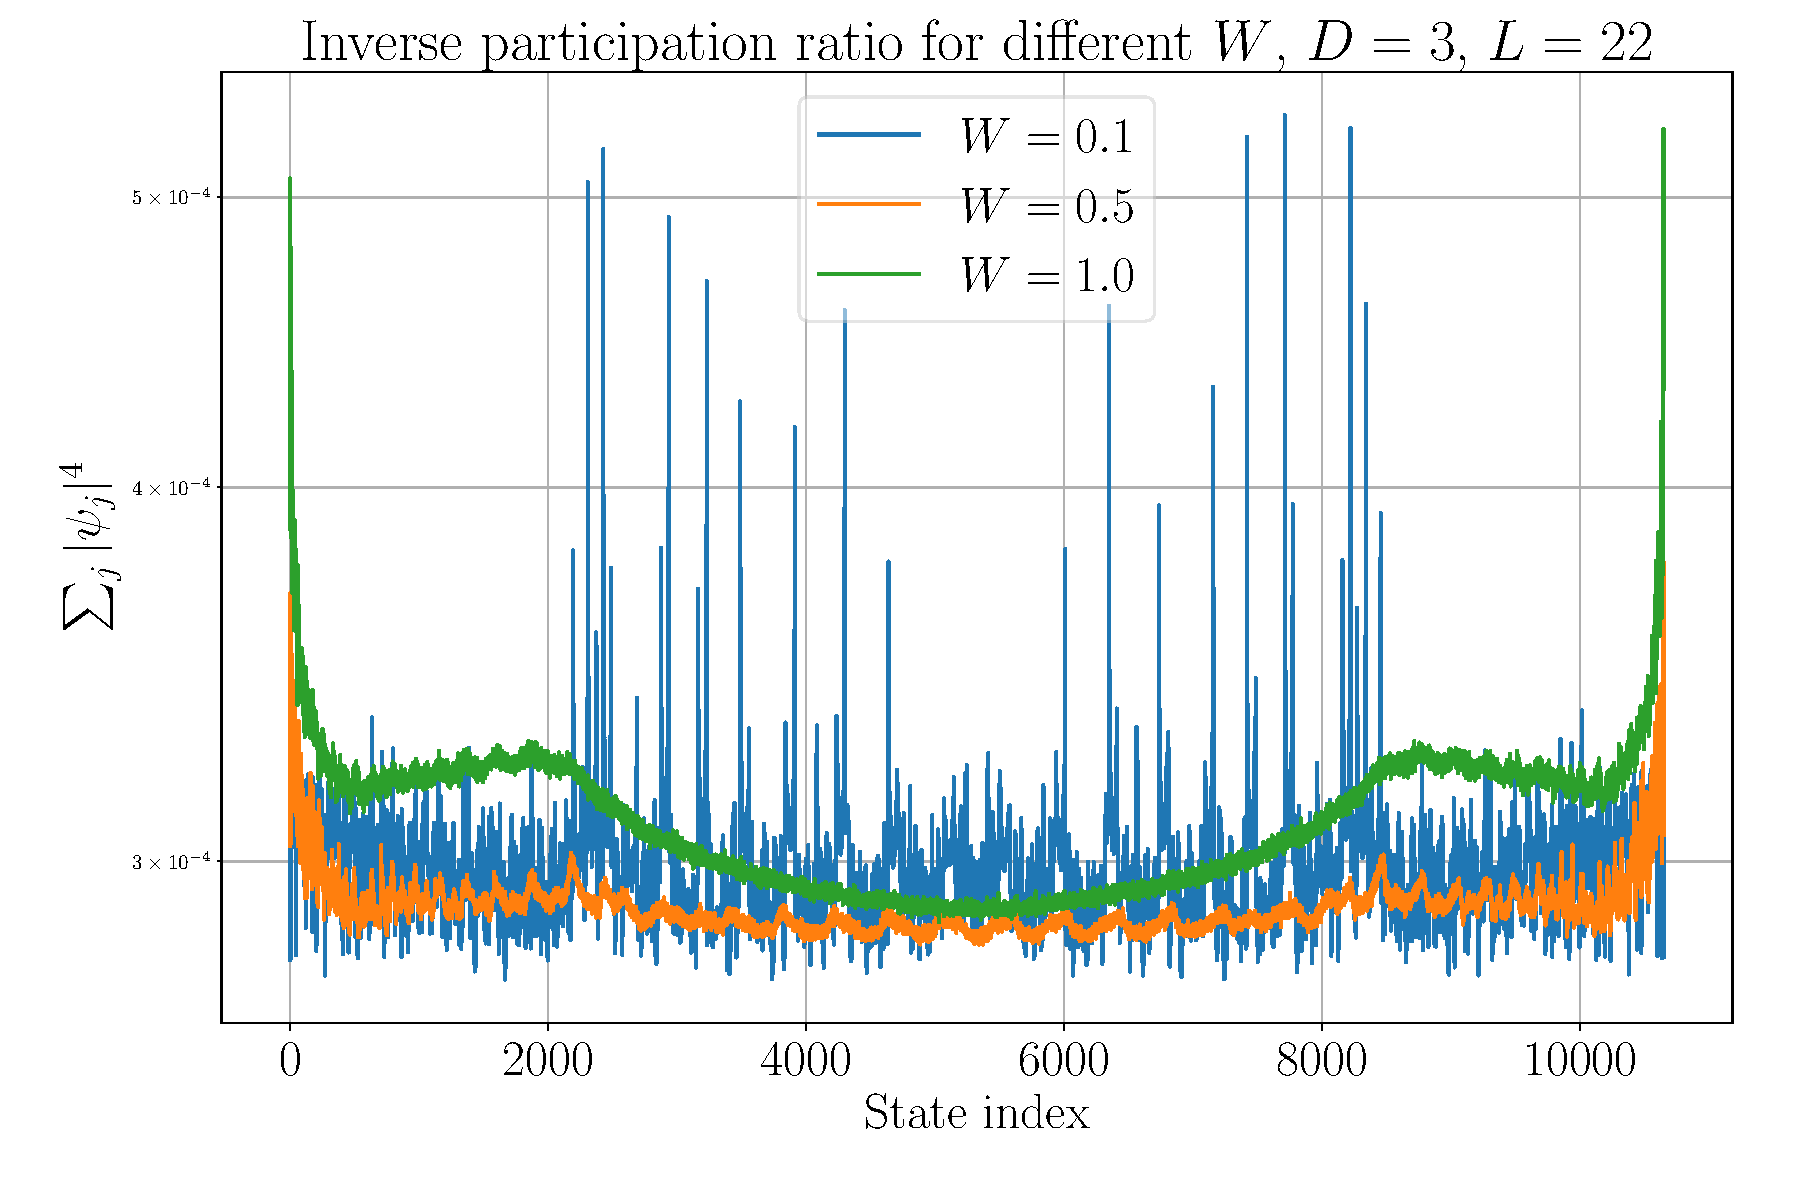
\includegraphics[width=0.62\textwidth]{3D_Anderson_localization_Seminar_scaling_analysis_D3_shape_22_22_22_eigensys_plots_single_presentation.pdf}}
\end{figure}
\subsection{The absence of diffusion}
We have already established that localized states cannot contribute to electron transport in a disordered system. An initial localized wavefunction $\ket{\psi, 0}$, which should not be an eigenstate of the Hamiltonian given by Eq. \eqref{eq:anderson}, will, after some transient time, not spread across the whole system with time if all eigenstates are localized. Quantitatively, its average diameter $\tilde{R}$ will saturate at some value smaller than the system size if the system is sufficiently large so that no finite-size effects occur.\\\\
\noindent 
In our numerical simulations, an initial wavefunction with considerable probability amplitude only at a few sites in the center of the lattice was time evolved with a unitary time-evolution operator according to the scheme given by Eq. \eqref{eq:propagation}. The wavefunction`s average diameter was determined by calculating the expectation value of the $\hat{R^2}$ operator, defined by
\begin{equation}\label{eq:spread}
\hat{R^2}=\sum\limits_{\mathbf{r}_j} \mathbf{r}_j^2 \hat{n}_{\mathbf{r}_j}, \hspace{10mm} R(t)=\sqrt{\bra{\psi,t} \hat{R^2}\ket{\psi,t}-\bra{\psi,0} \hat{R^2}\ket{\psi,0}},
\end{equation}
where $\hat{n}_{\mathbf{r}_j}=c^\dagger_{\mathbf{r}_j}c_{\mathbf{r}_j}$ is the particle number operator at the site $\mathbf{r}_j$. In the fully localized case, $R(t)$ eventually saturates at a finite value. In the absence of disorder, on the other hand, the transport is ballistic with $R(t)=\sqrt{zV}t$ for an initial wavefunction where a particle is located at a single site. Only these two possibilities exist in 1D and 2D, while an additional intermediate diffusive regime is possible in 3D for subcritical disorder when both extended and localized states exist in the system. The time dynamics simulations have been performed in 1D and 2D and their results are shown below.   \\\\
\noindent 
\begin{minipage}[t]{0.27\textwidth}
Time evolution of an initial delta-like probability distribution centered at the $j=0$ site in a 1D lattice is shown in Fig. \ref{fig:light_cone}. The evolution was performed in the regime of no disorder and in the regime of strong disorder with $W=0.$ The ballistic spread is clearly evident in the former case with the wave function's average diameter growing linearly in time. In the second case, the probability amplitude remains peaked in the vicinity of its initial site, spreading only minimally, which is a hallmark of localization. A more detailed study of the time-dynamics in 1D is shown in Fig. \ref{fig:1D_rsq}.
% We note that finite-size effects represent a formidable challenge in the studies of time-dynamics as well, especially in the limit of weak disorder in 1D and 2D. As shown in Fig. \ref{fig:1D_rsq}, in the $W=0.1$ case, a wave packet might reach the lattice edges before it had stopped spreading. This might lead one to misinterpred the result as a hallmark of absence of localization, whereas localization actually occurs, only on a length scale greater than the system size. Since we were unable to tackle the finite-size effects by increasing the
\end{minipage}\hfill
\begin{minipage}[t]{0.72\textwidth}
\begin{figure}[H]
\centering{
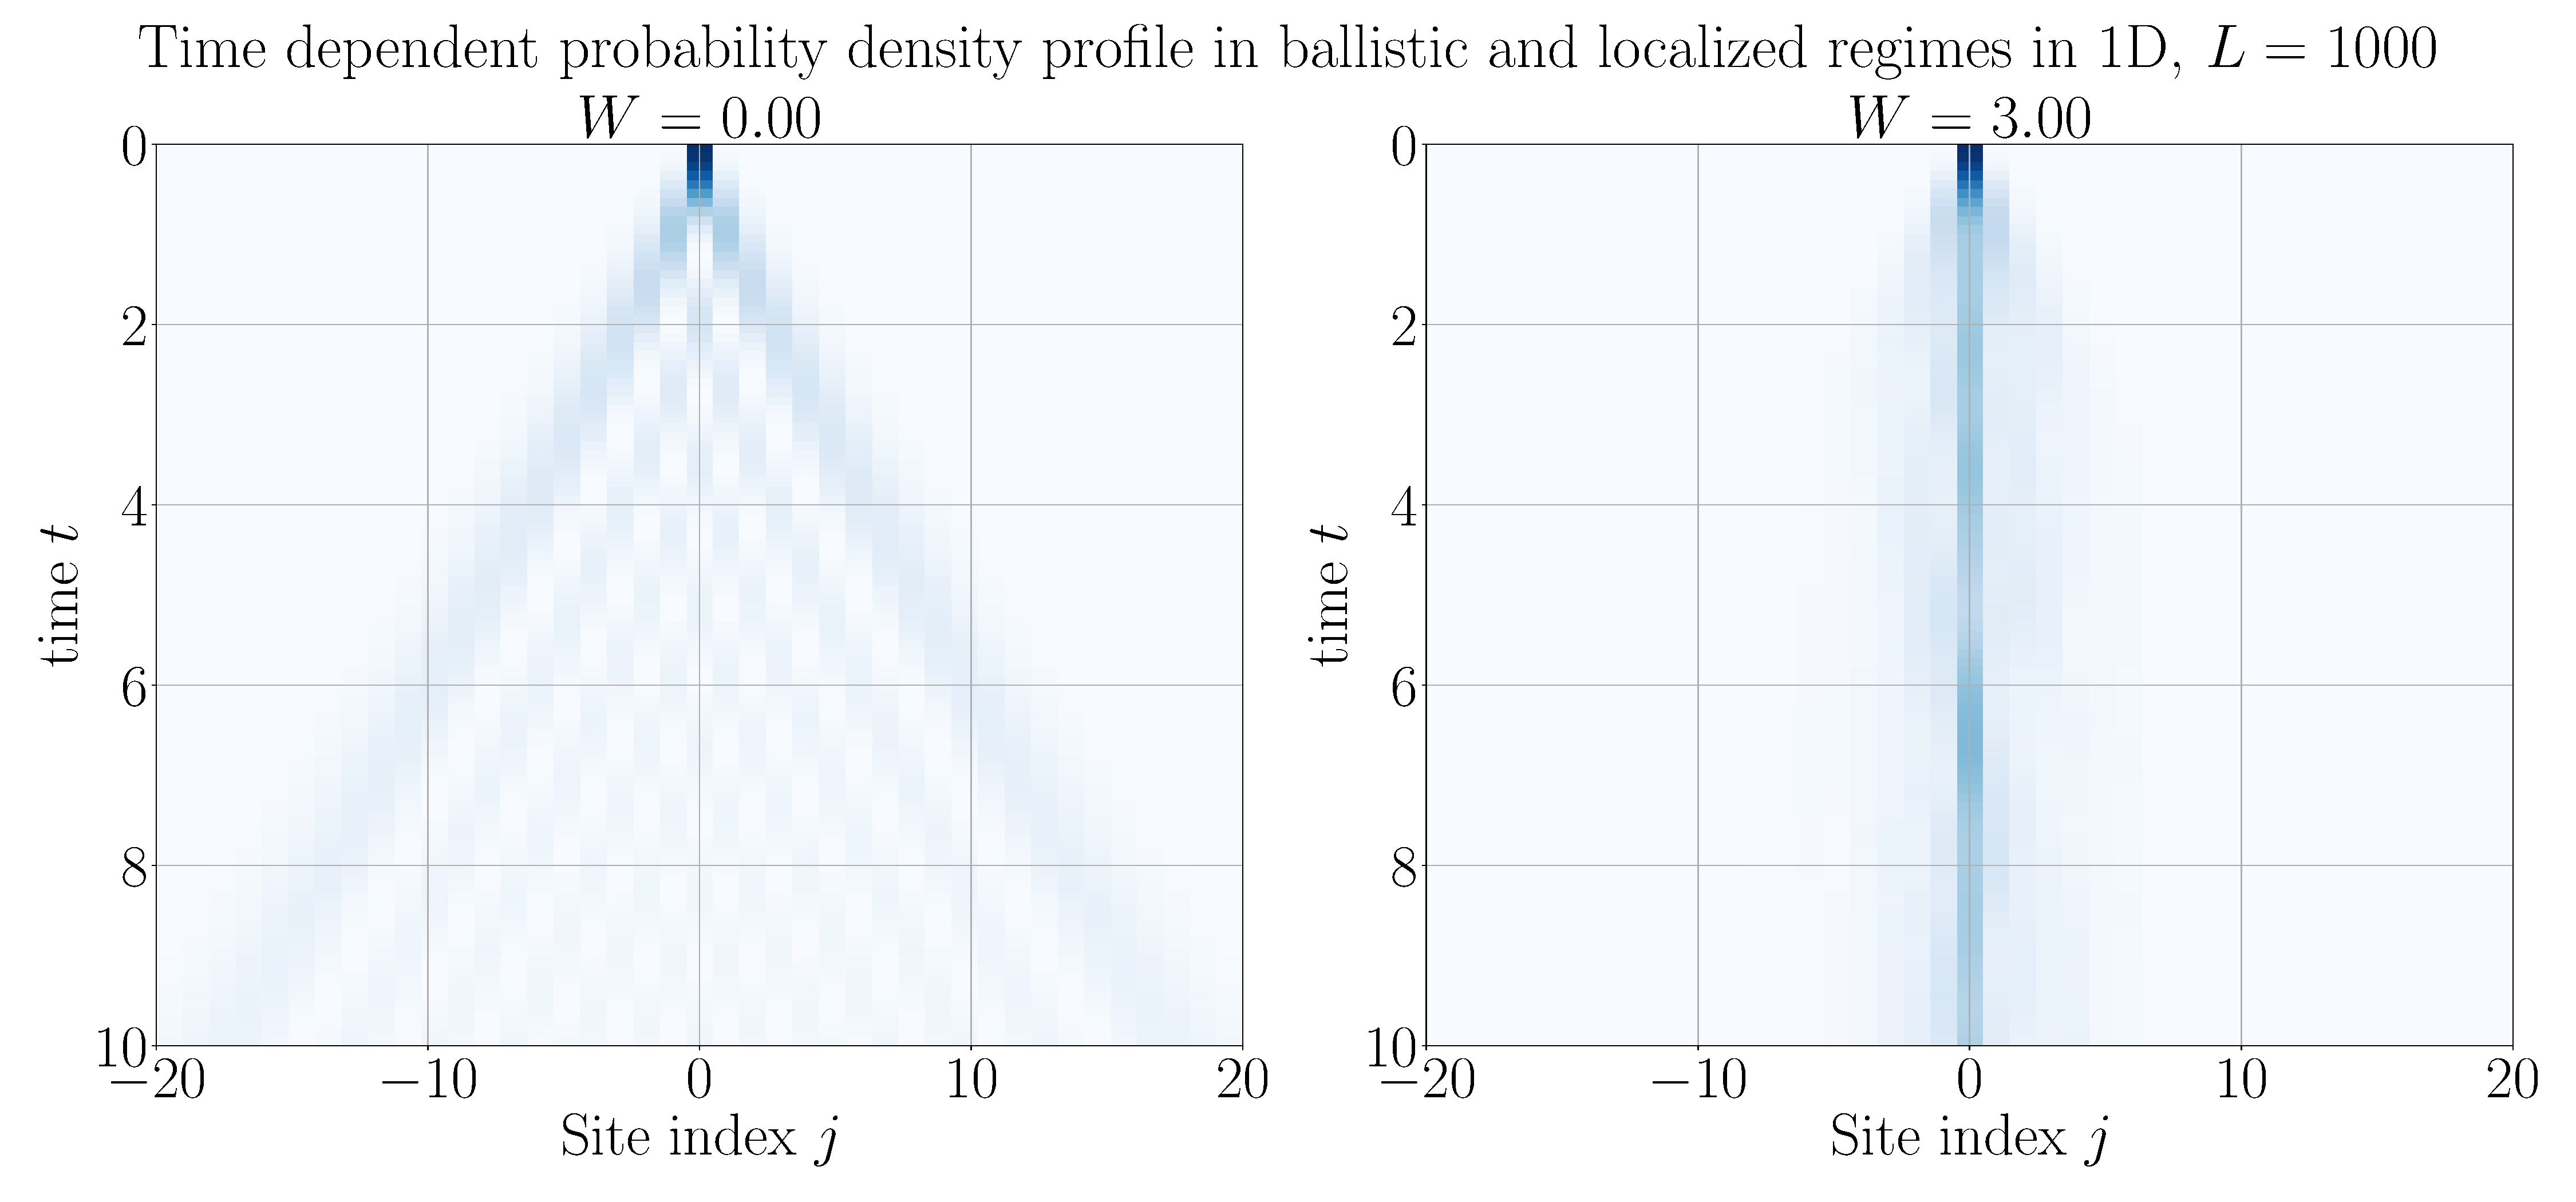
\includegraphics[width=1\textwidth]{1D_Anderson_loc_seminar_D1_shape_1000_light_cone_double.pdf}}
\caption{Time evolution of an initial delta-function like wave packet in the ballistic regime with $W=0.0$ and in the localized regime with $W=3.0$ where all eigenstates are localized due to strong disorder. While the density profile spreads out with time in the first case it remains localized around its initial site $j=0$ in the second case. }
\label{fig:light_cone} 
\end{figure}
\end{minipage}\\\\
An analysis of the time evolution data has been performed by considering the time dependence of the scaling exponent $\beta(t)$ in the leading term of the $R(t)$ dependence:
\begin{equation}\label{eq:beta_time}
R(t)\approx At^{\beta(t)}+\dots, \hspace{1cm} \beta(t)=\frac{\dd \log R(t)}{\dd \log t}.
\end{equation}
The derivative in the expression for $\beta(t)$ has been estimated numerically using discrete finite differences. In the ballistic regime, the value of $\beta$ is identically equal to one at all times, whereas it should monotonically decrease with time towards the value of zero in the localized case when the saturation of $R(t)$ at some finite value is expected.  
% Absence of diffusion in the presence of disorder was studied by time evolving an initial sharply localized wave packet according to the propagation scheme \eqref{eq:propagation} and evaluating the value of $R(t)$ given by Eq. \eqref{eq:spread} on each propagation step. Numerical package \url{sparse} for calculations involving sparse matrices from \url{Python} \url{SciPy} library has been used in our calculations since the Anderson Hamiltonian can be represented by a sparse matrix. The time-evolution operator in Eq. \eqref{eq:propagation} has been approximated by its Taylor expansion up to tenth order which proved sufficiently accurate for our calculations. The wavefunction $\ket{\psi,t}$ was renormalized on each time step to make sure that the propagation preserved its norm. 	A step-length of $\dd t=0.1$ has been used in all time-evolution simulations. \\\\\\\\
\noindent 
The value of $\beta$ is identically equal to 1 at all times in the ballistic case and should monotonically decrease in time towards the value of zero for any finite disorder. In actual simulations, this only holds true for as long as the finite-size effects are absent. An estimate for the smallest time interval on which the propagation is free of finite-size effects is obtained by considering the $W=0$ case in which the Anderson Hamiltonian is a simple tight-binding Hamiltonian. In that case, the initial wave function can be expanded in the Fourier basis of Bloch states and the time estimate is obtained by dividing the separation between the initial site and the edge boundary by the velocity of the fastest Fourier component in the expansion, which equals $v_\mathrm{max}=zV$ in the tight-binding case. For an initial site in the lattice center, the distance to the edge boundary equals $L/2$, so we have $t_\mathrm{max}=\frac{L}{2zV}$, where we have set both the lattice constant and reduced Planck's constant $\hbar$ to unity.
\\\\
\noindent 
We note that $\beta(t)=\frac{1}{2}$ equality corresponds to the diffusive case which is supposed to occur in 3D. The results of the simulations in the 1D and 2D case are shown in Figs. \ref{fig:1D_rsq} and \ref{fig:2D_rsq}.\\\\
\begin{figure}[H]
\centering{
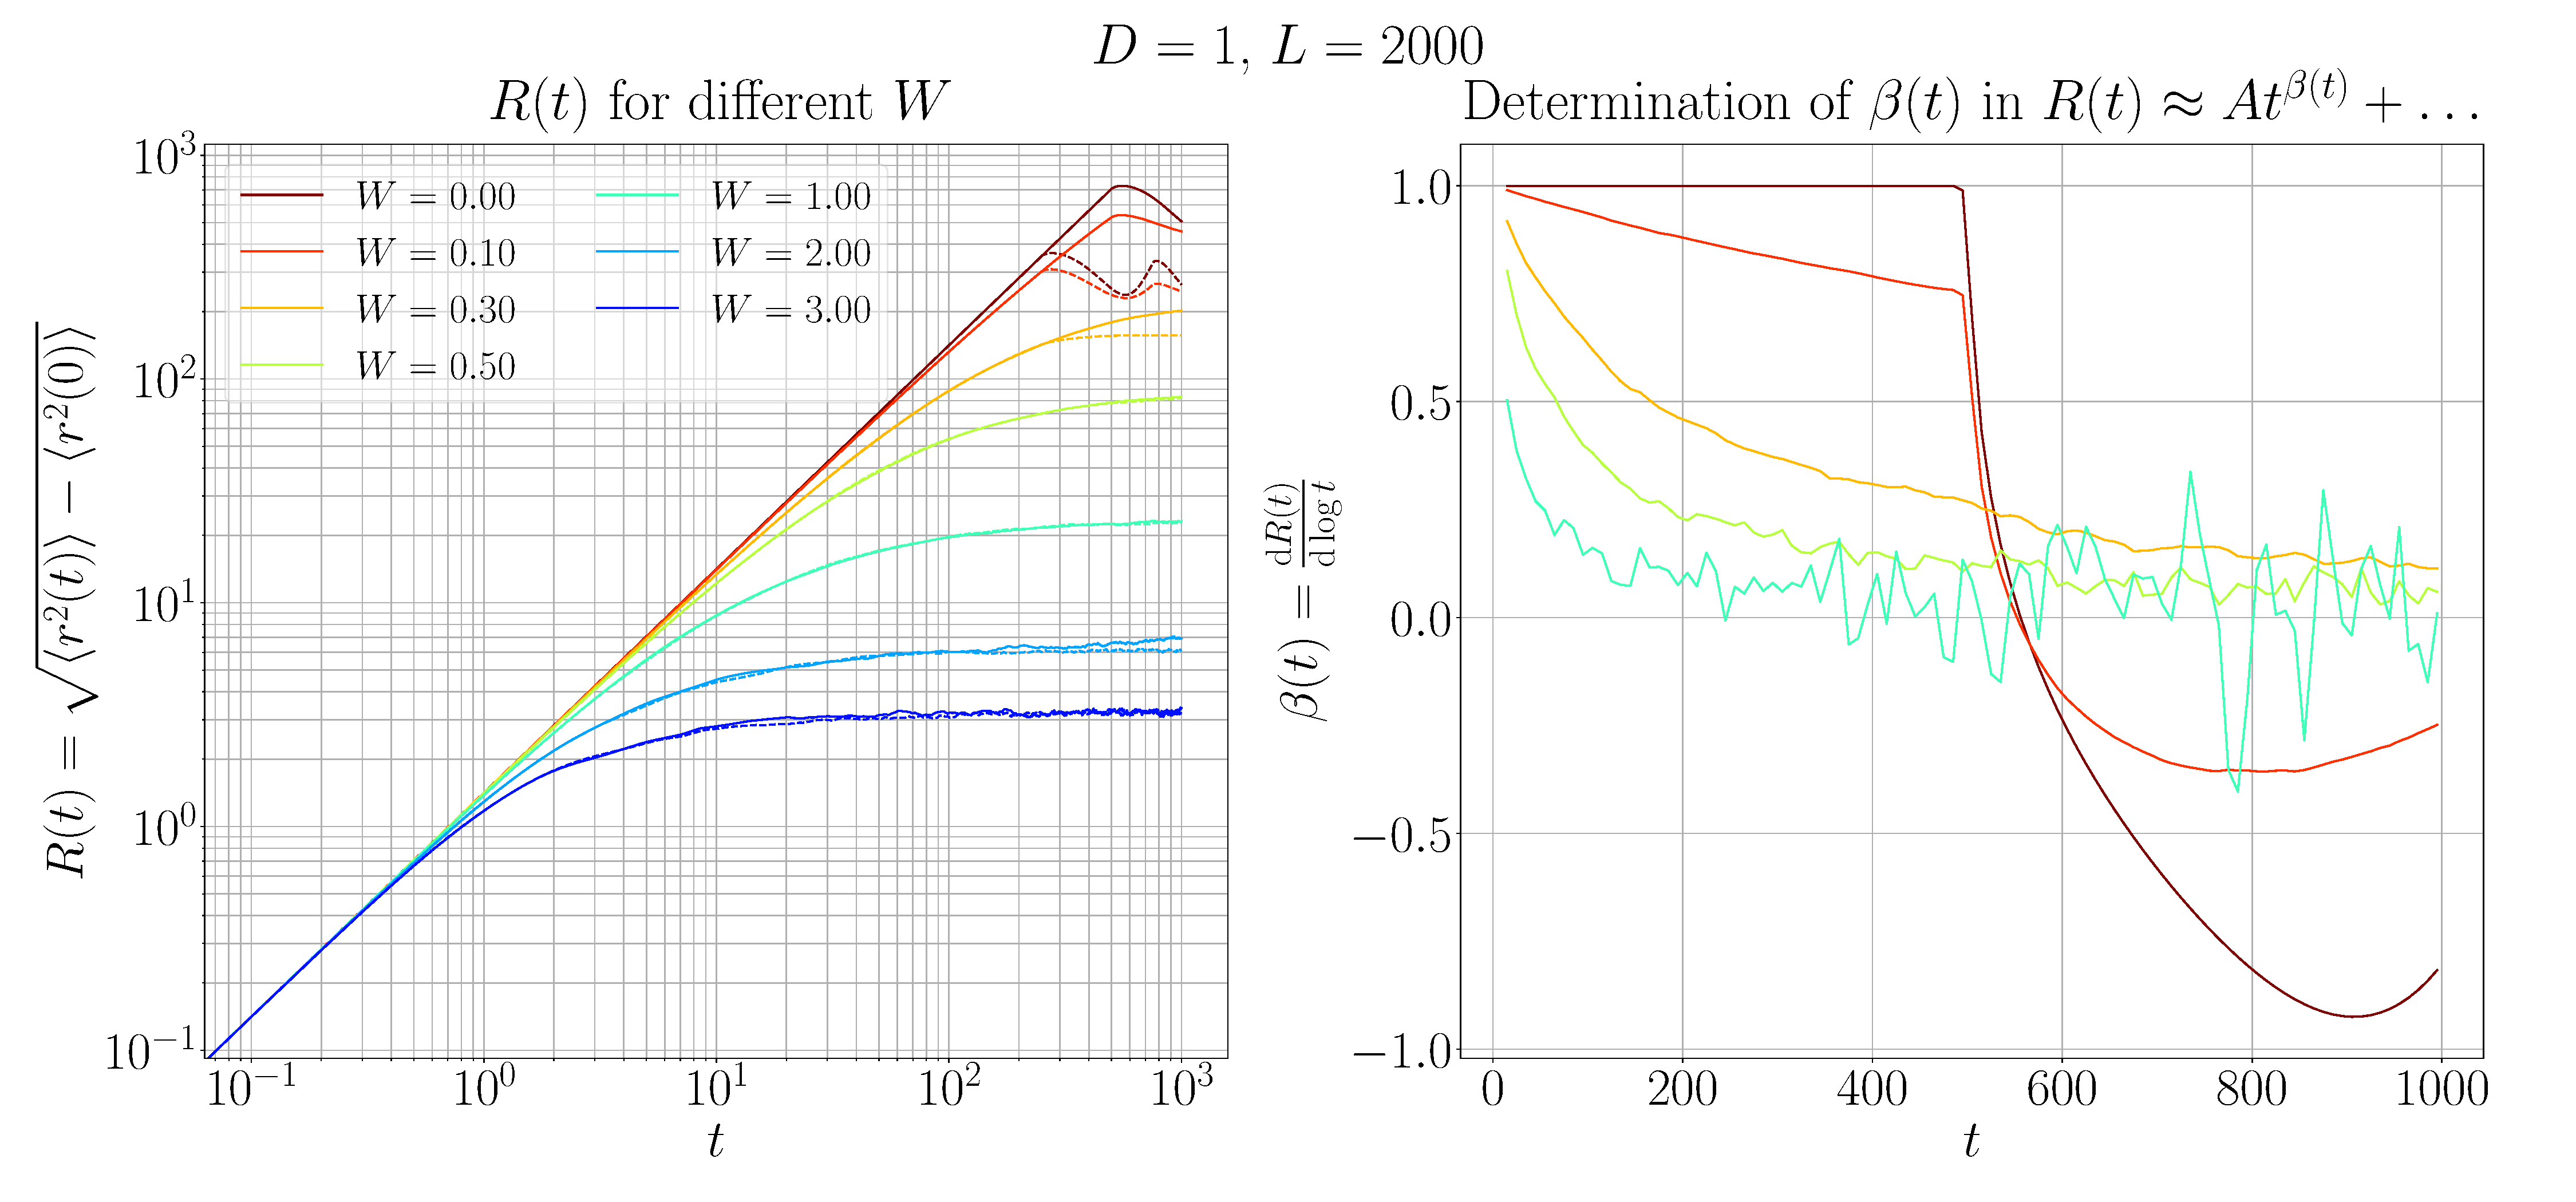
\includegraphics[width=0.9\textwidth]{1D_Anderson_localization_Seminar_scaling_analysis_D1_shape_2000_r_sq_dynamics.pdf}}
\caption{One-dimensional lattice with $L=2000$ sites. Left: time dependence of $R(t)$ averaged over 200 realizations of disorder for different values of $W$. Finite size effects are prominent in the $W=0.0$ and $W=0.1$ case, leading to a decrease in $R$ at around $t_\mathrm{max}=500$ when the wave packets reached the lattice boundaries. The results for the three highest values of disorder clearly show a saturation value was reached. Dashed lines show the results of simulations on a lattice with $L=1000$ sites. Right: numerical approximation of $\beta(t)=\frac{\dd \log R(t)}{\dd \log t}$. A decreasing trend towards the value of zero is evident for finite disorder.  While curves for values of $W<1.0$ seem rather smooth, the $W=1.0$ curve shows strong fluctations, implying averaging should be performed over a greater number of samples for large $W$. Again, the $W=0.0$ and $W=0.1$ curves are only physically relevant up to $t=500$ due to finite-size effects. }
\label{fig:1D_rsq} 
\end{figure}
\noindent 
% \begin{figure}[H]
% \floatbox[{\capbeside\thisfloatsetup{capbesideposition={left,center},capbesidewidth=2.3cm}}]{figure}[\FBwidth]
% {\caption{Left: time dependence of $R(t)$ for different values of $W$. Finite size effects are prominent in the $W=0.0$ and $W=0.1$ case }\label{fig:1D_rsq}}
% {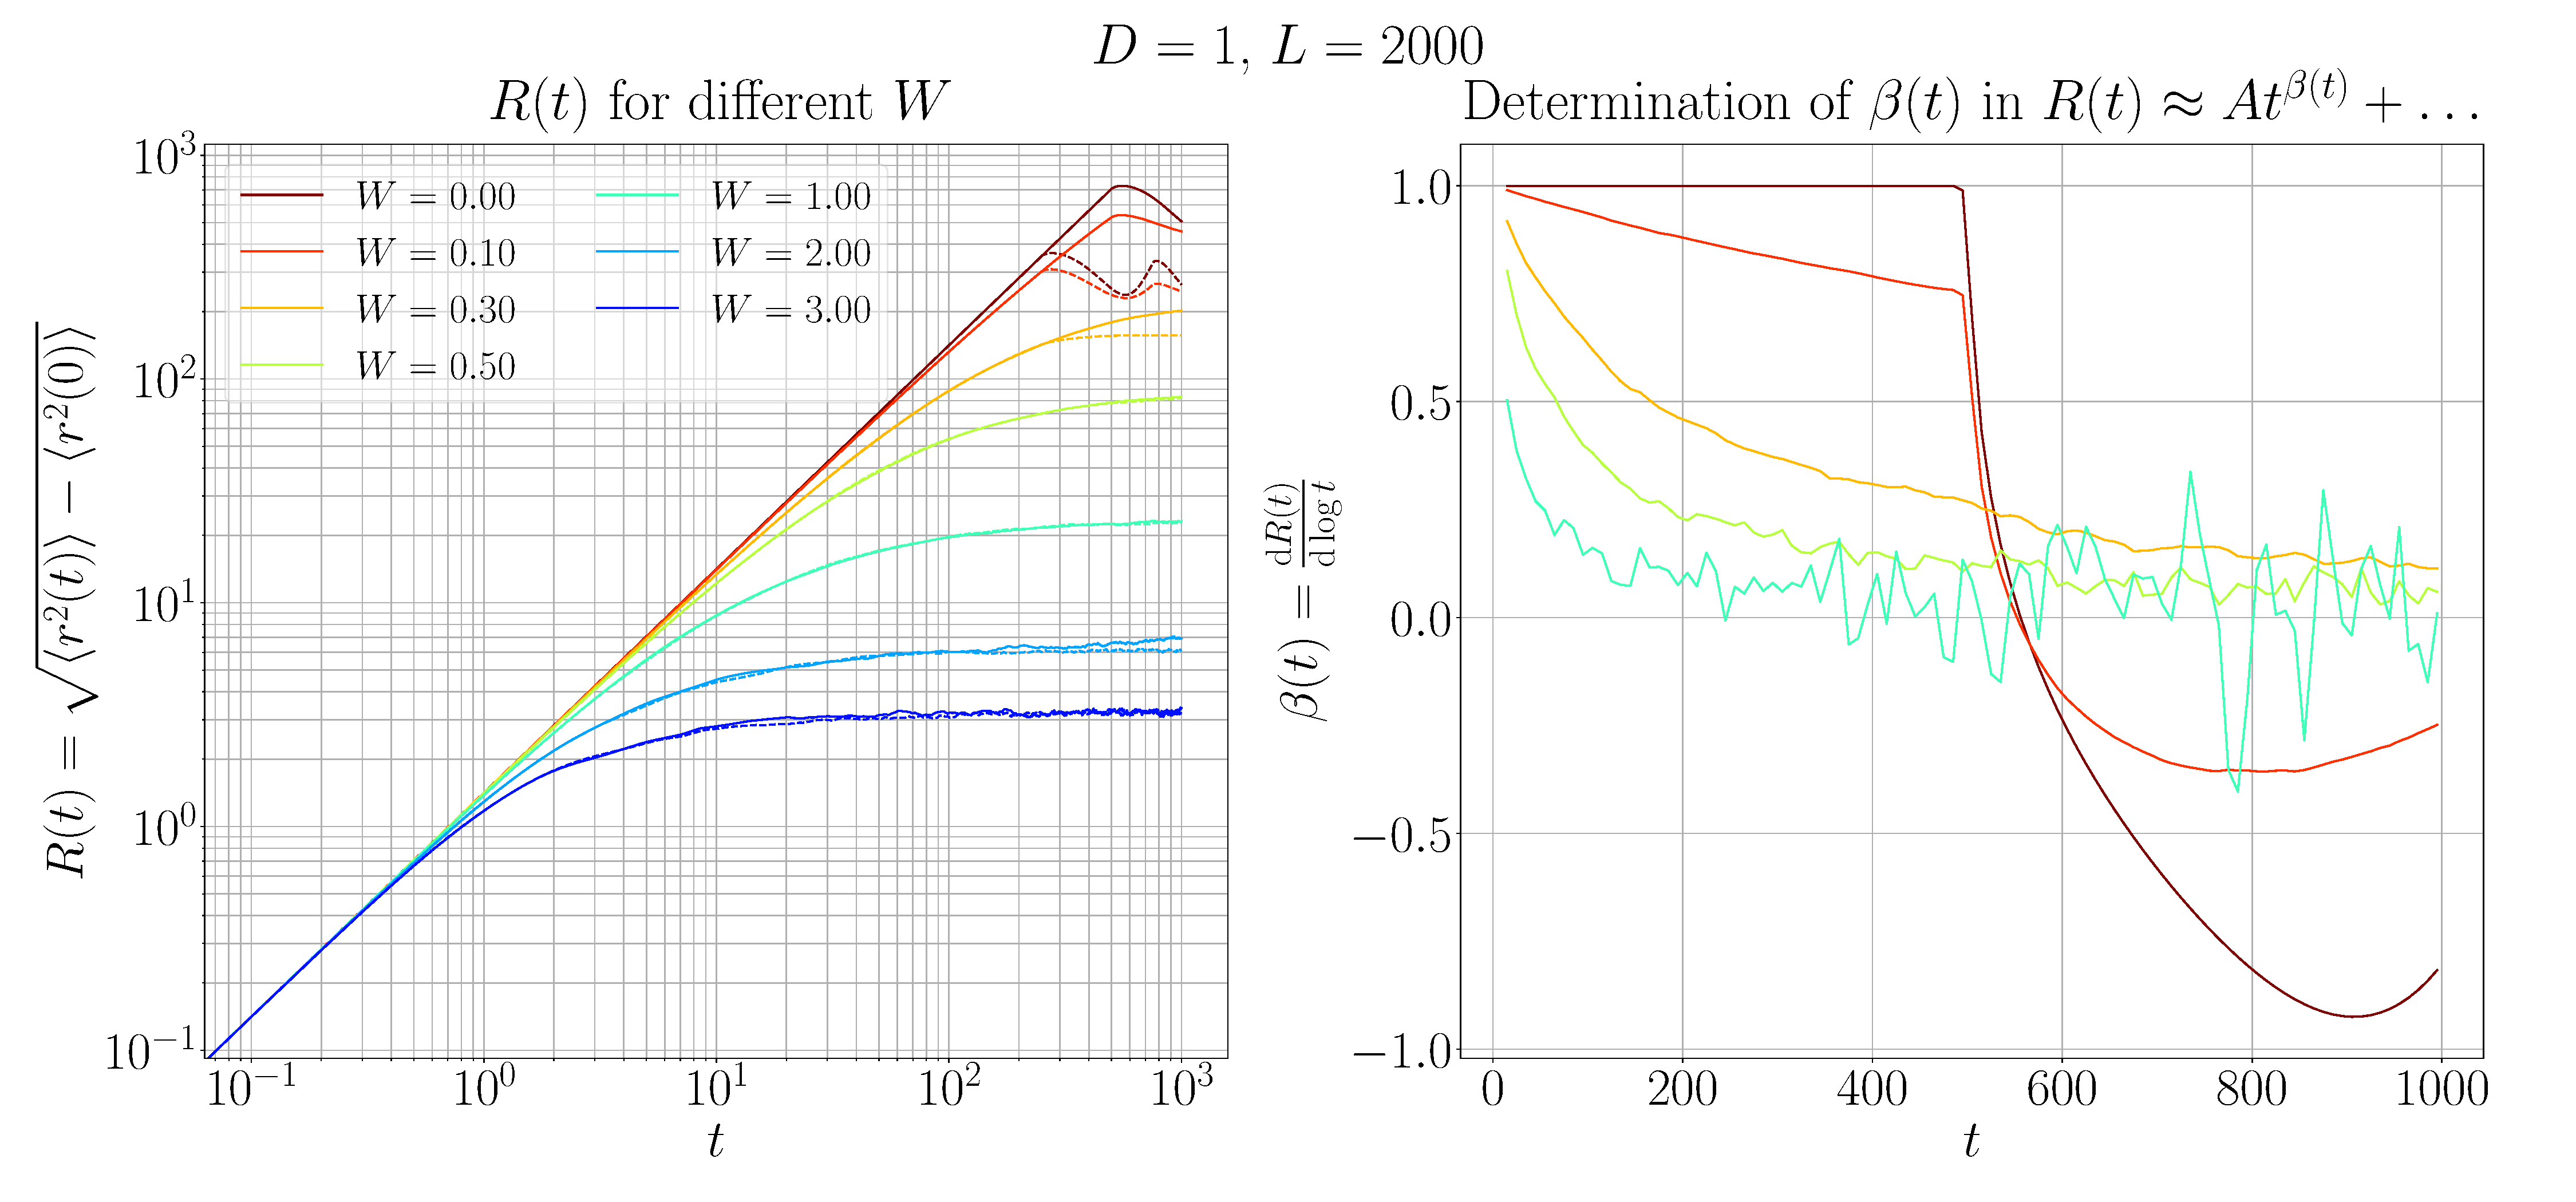
\includegraphics[width=0.85\textwidth]{1D_Anderson_localization_Seminar_scaling_analysis_D1_shape_2000_r_sq_dynamics.pdf}}
% \end{figure}
% \begin{figure}[H]
% \floatbox[{\capbeside\thisfloatsetup{capbesideposition={left,center},capbesidewidth=2.3cm}}]{figure}[\FBwidth]
% {\caption{ }\label{fig:1D_ipr}}
% {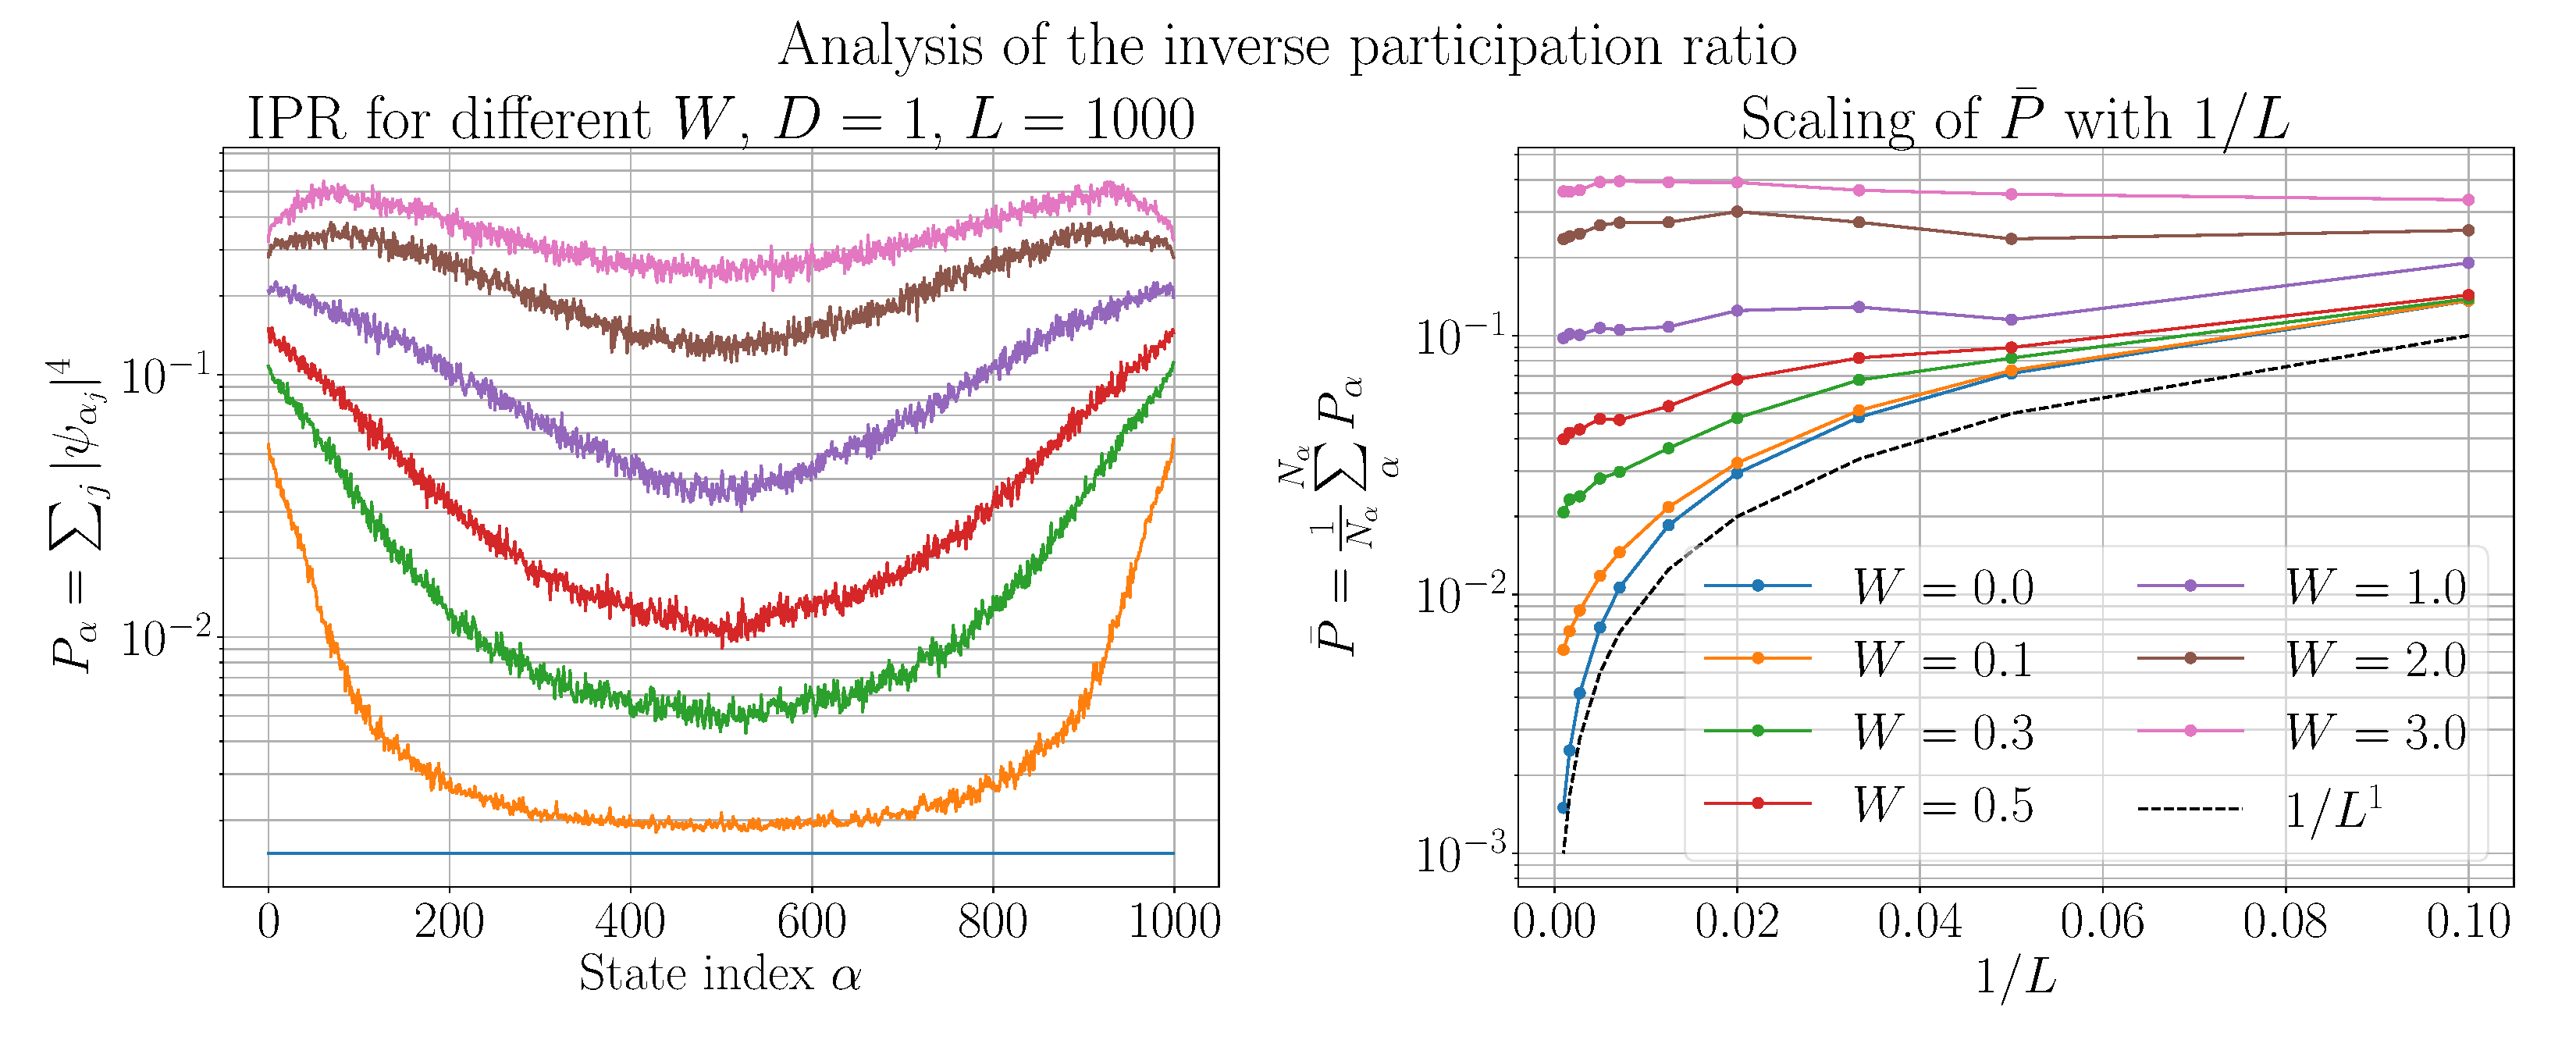
\includegraphics[width=1\textwidth]{1D_Anderson_localization_Seminar_scaling_analysis_D1_shape_1000_ipr_plots.pdf}}
% \end{figure}
\begin{figure}[H]
\floatbox[{\capbeside\thisfloatsetup{capbesideposition={left,center},capbesidewidth=3.cm}}]{figure}[\FBwidth]
{\caption{Two-dimensional lattice with $500\times500$ sites. Compared to the one-dimensional case shown in Fig. \ref{fig:1D_rsq}, it takes longer for $R(t)$ to saturate and the finite-size effects are more prominent since lattice boundaries can be reached sooner. Averaging was performed over 50 realizations of disorder.}\label{fig:2D_rsq}}
{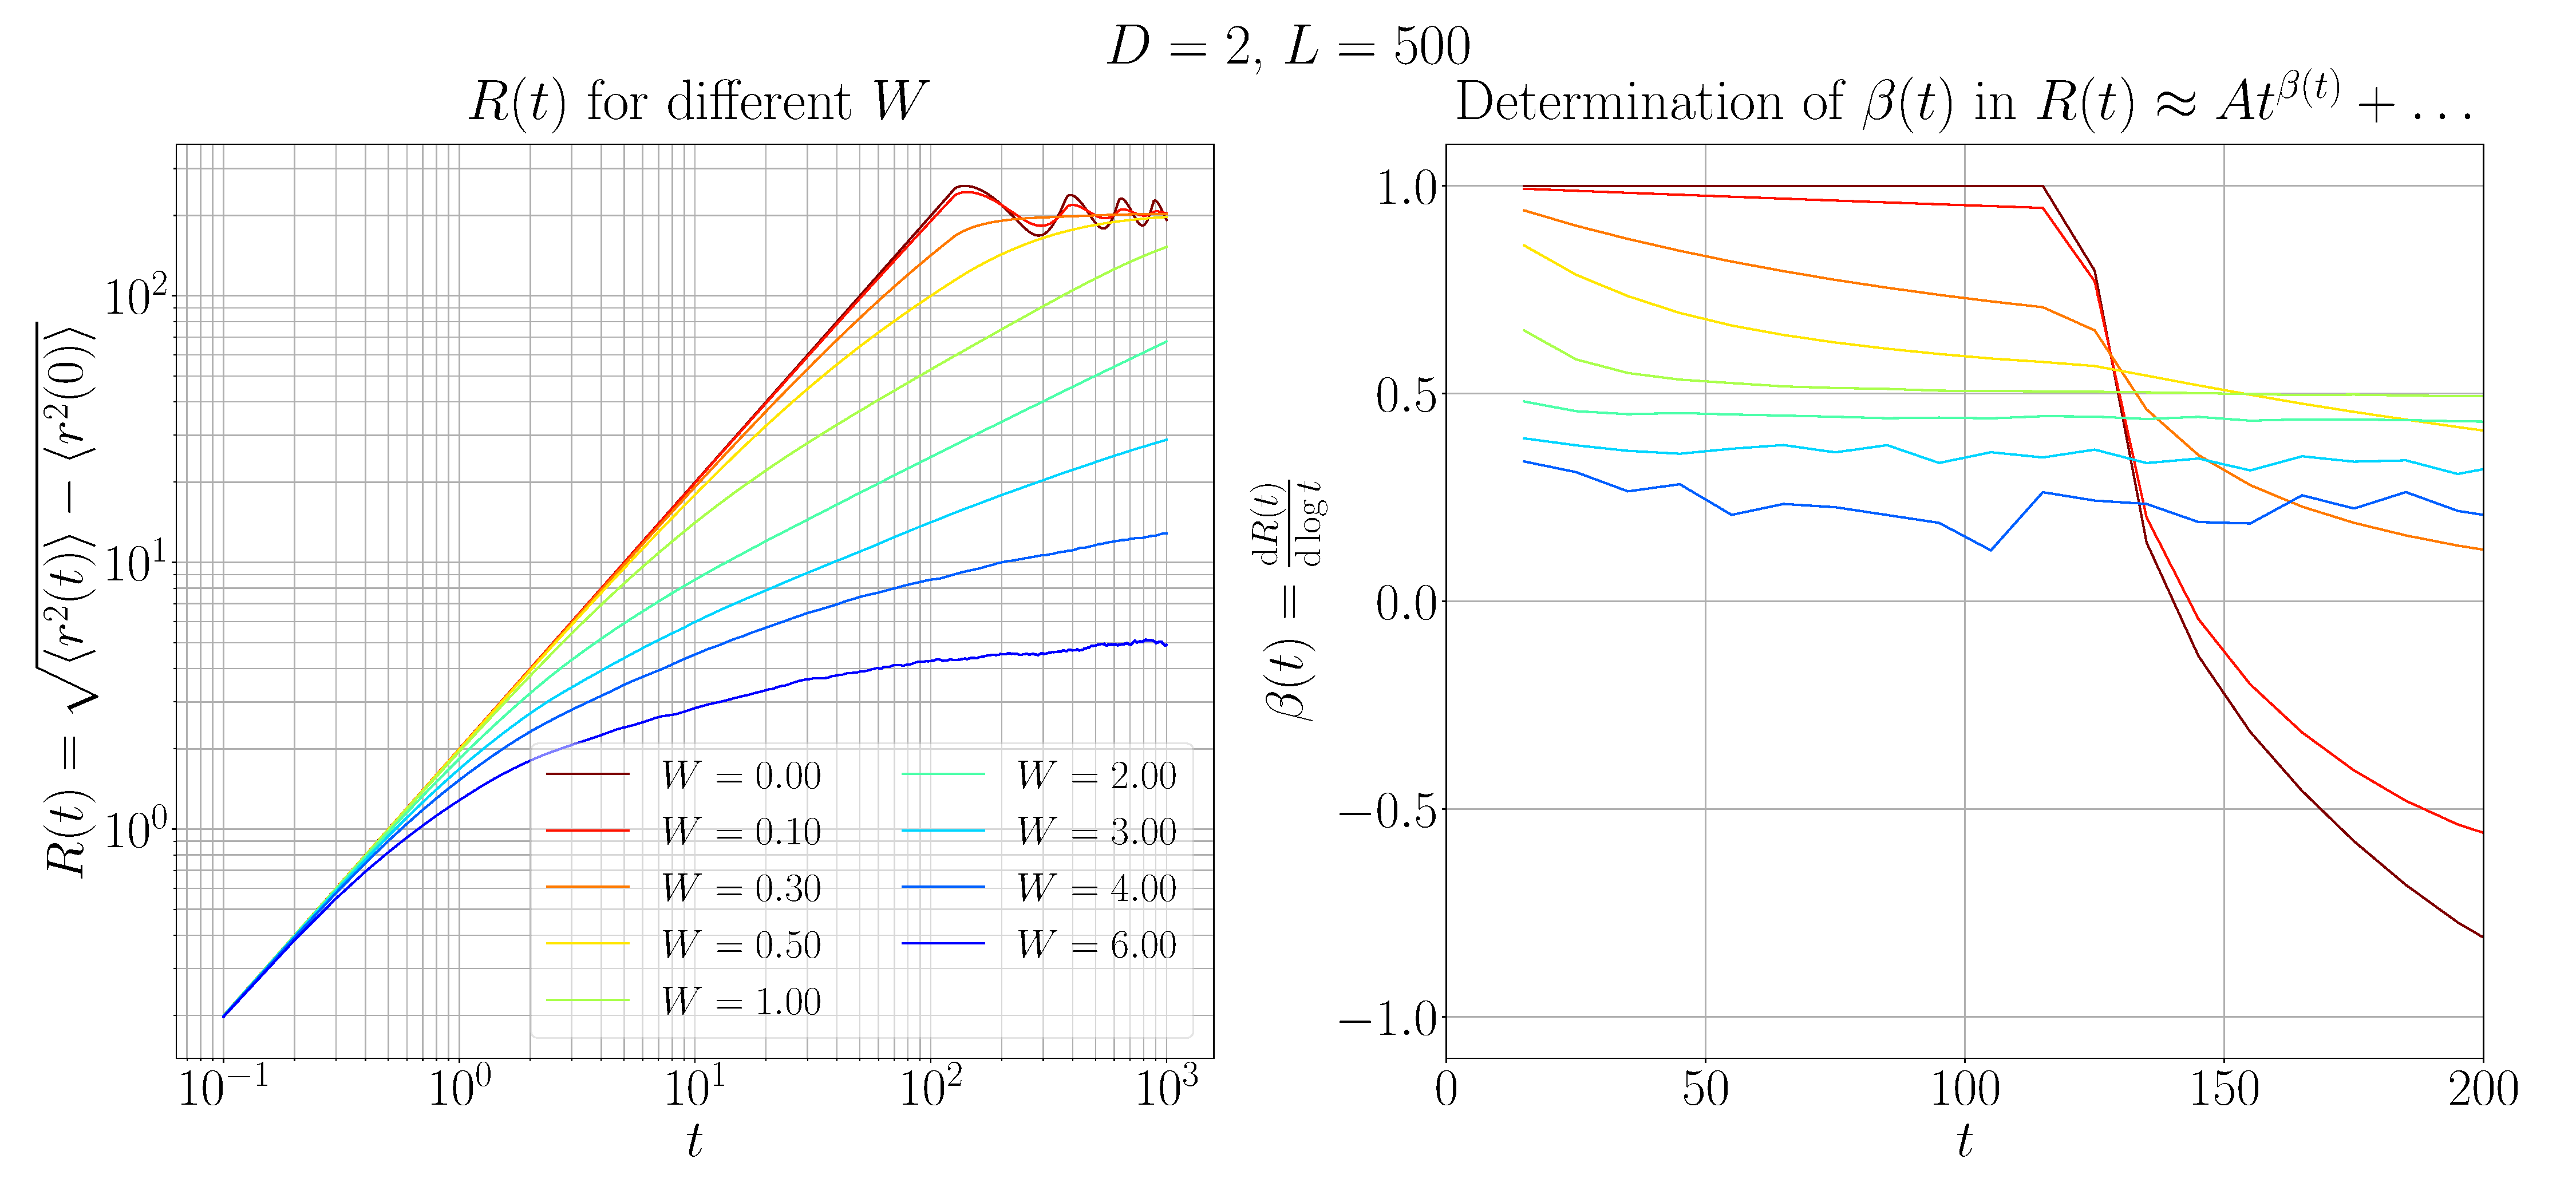
\includegraphics[width=0.8\textwidth]{2D_Anderson_localization_Seminar_scaling_analysis_D2_shape_500_500_r_sq_dynamics.pdf}}
\end{figure}
\noindent 
To conclude the section, we have shown that the characteristic signatures of localization are clearly evident in the 1D case both in the decaying $\beta(t)$ dependence and in the finite-size scaling of $\bar{P}$. The same features are also present in the 2D results, however, some ambiguity remains in the limit of small $W$, which we could not resolve. This is in large part due to the memory constraints which prevented us from performing finite-size scaling analysis and time evolution on larger systems. Studies of the inverse participation ratio in 3D confirm the existence of two mobility edges while a more detailed analysis has not yet been attempted.  
\section{Conclusion}
\label{sec:conc}
The phenomenon of Anderson localization and the numerical implementation of the Anderson Hamiltonian have been presented in this seminar. In stark contrast to the preceeding models of electron conduction, the localization theory correctly predicted the vanishing of conductivity in a three-dimensional system with sufficiently strong disorder, thus allowing for a development of a more complete description of transitions between metals and insulators in real systems. The existence of such a theory is of particular importance since at least some degree of disorder is usually present in the actual systems. As shown in the seminar, the localization phenomena depend nontrivially on the dimensionality of the system under consideration. Only localized states exist in 1D and 2D for any nonzero disorder, while a transition between the insulating and the metallic regime is possible in 3D. Still lacking a complete theoretical treatment, the progress in the field of localization depends invaluably on the results of the numerical simulations. Their implementation is highly nontrivial, especially in 3D, as also the numerical work presented in this seminar illustrates. Finally, we note that understanding localization in non-interacting systems is a precondition for understanding the many-body localization (MBL) phenomena which occur in the systems of interacting particles. Once the interactions are introduced, the physics presented in this seminar becomes even more complex which is why MBL is among the hot topics of recent research with many open questions still waiting to be answered. 
% \begin{figure}[H]
% \centering{
% 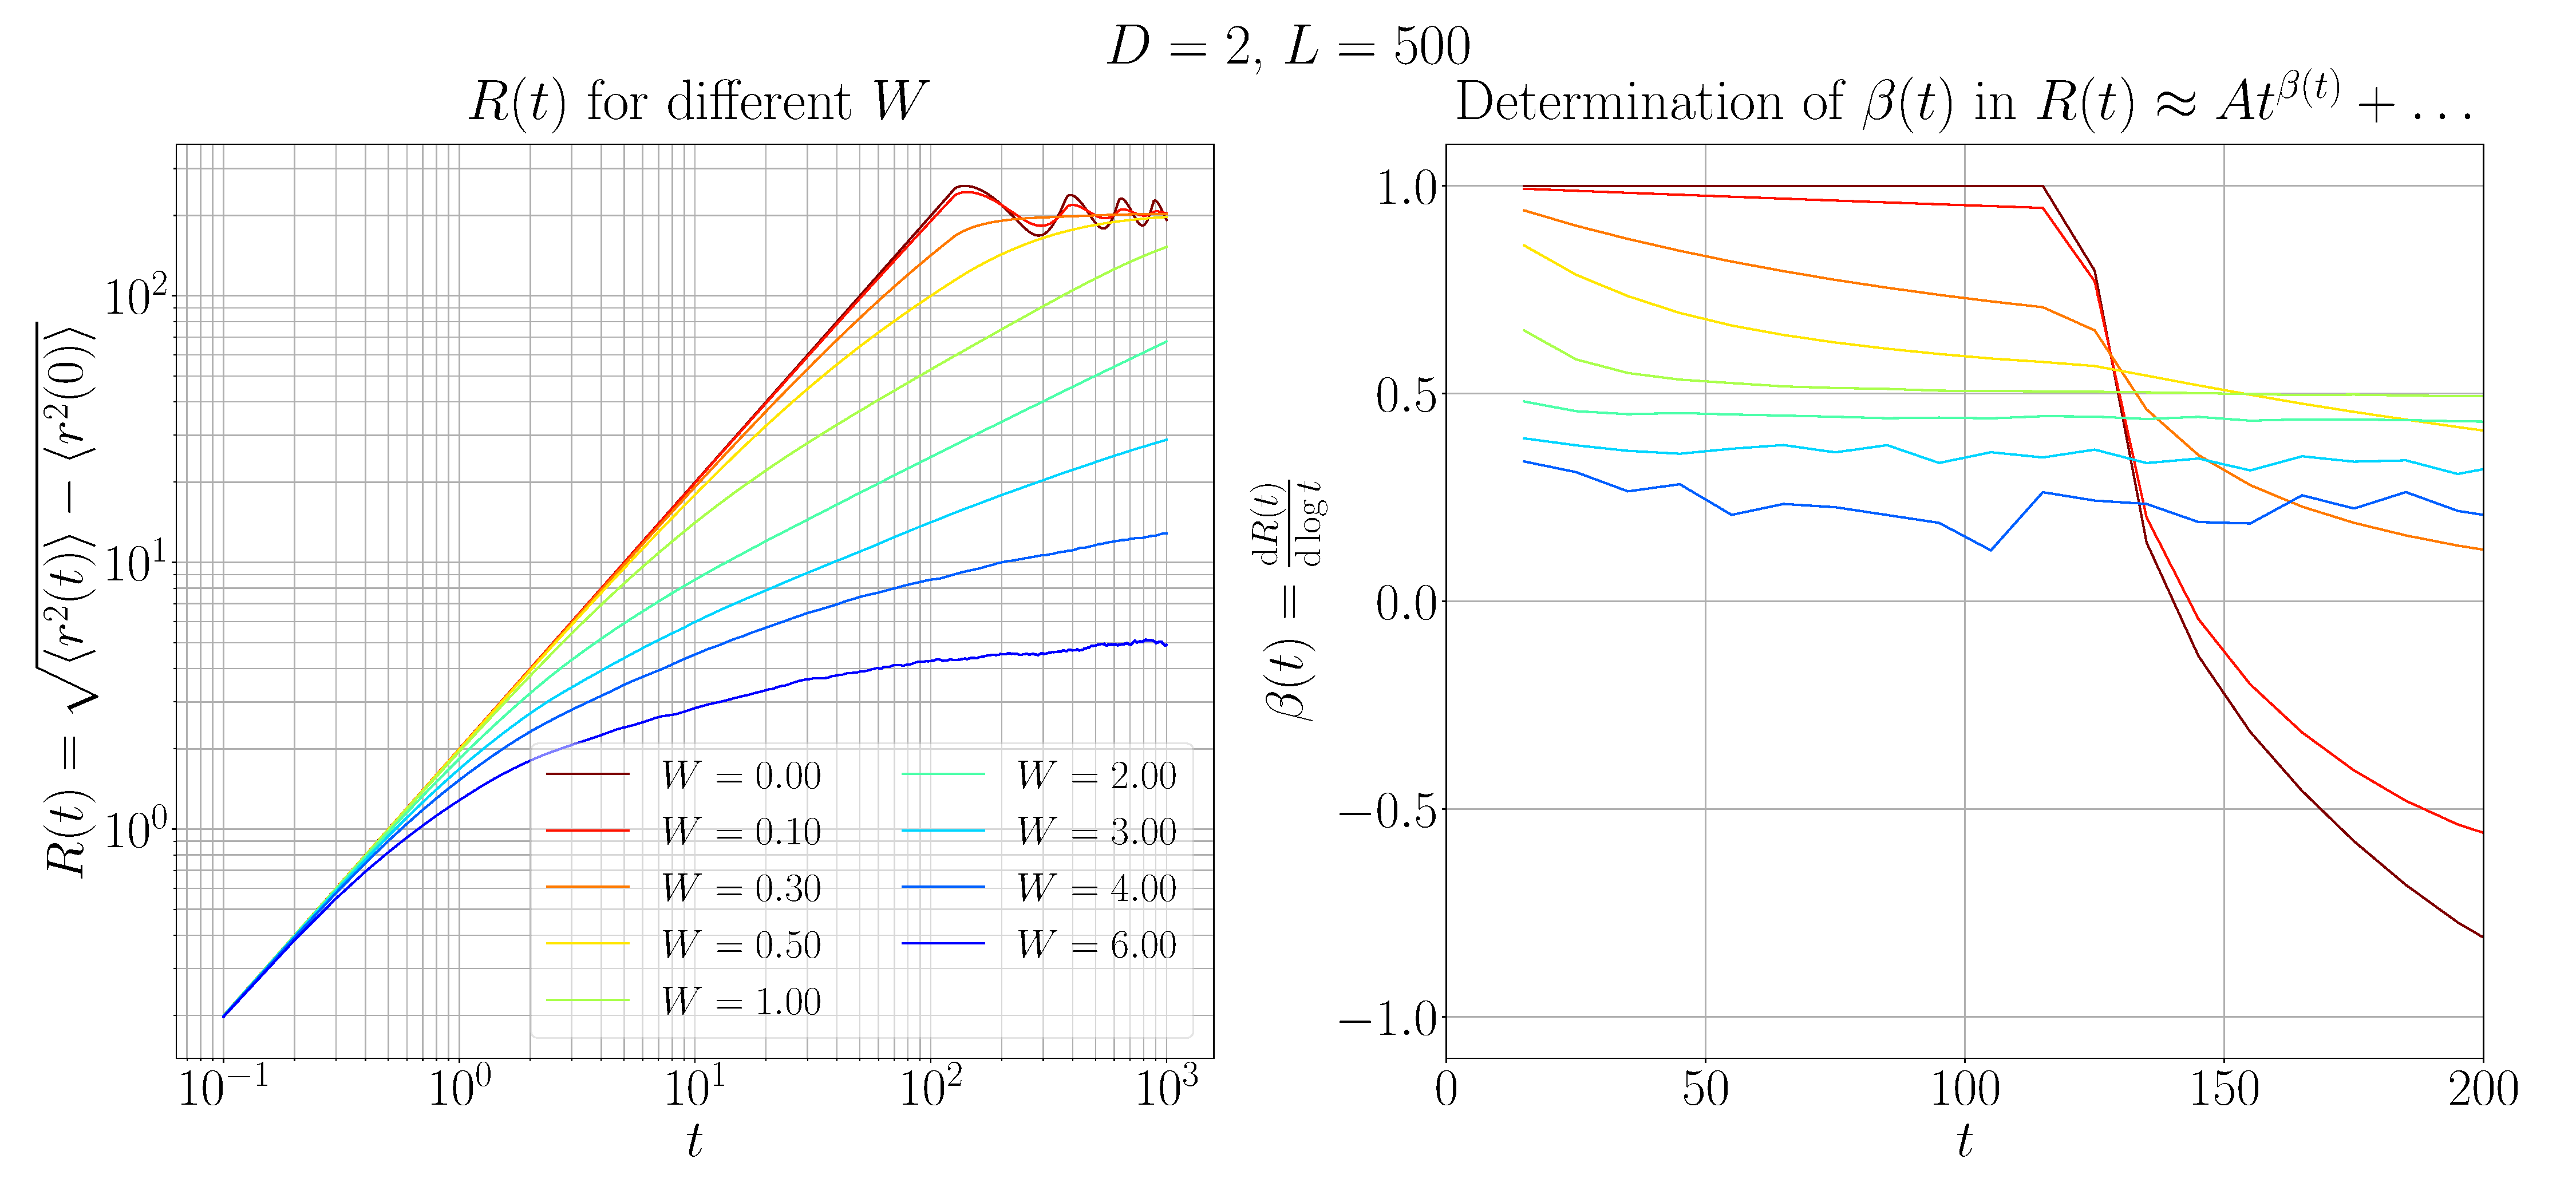
\includegraphics[width=0.8\textwidth]{2D_Anderson_localization_Seminar_scaling_analysis_D2_shape_500_500_r_sq_dynamics.pdf}}
% \caption{}
% \label{fig:2D_rsq} 
% \end{figure}
\begin{thebibliography}{99}
\bibitem{Kramer}
Kramer, B. and MacKinnon, A. (1993). \emph{Localization: theory and experiment.} Reports on Progress in Physics, \textbf{56}(12), pp.1469-1564.
\bibitem{Anderson}
Anderson, P. (1958). \emph{Absence of Diffusion in Certain Random Lattices.} Physical Review, \textbf{109}(5), pp.1492-1505.
\bibitem{Mott_Twose}
Mott, N.F and Twose, W.D (1961). \emph{Adv. Phys.} \textbf{10}, 107
\bibitem{Mott_transitions}
Mott, N. (1978). \emph{Metal–insulator transitions}. Physics Today, \textbf{31}(11), pp.42-47.
\bibitem{scaling}
Abrahams E., Anderson P. W., Licciardello, D. and Ramakrishnan, T.V. (1979).\emph{Scaling Theory of Localization: Absence of Quantum Diffusion in Two Dimensions.} Phys. Rev. Lett. \textbf{42}(10), 673
\bibitem{self-consistent}
Wölfle, P. and Vollhardt, D. (2010). \emph{Self-Consistent Theory of Anderson Localization: General Formalism and Applications.} International Journal of Modern Physics B, \textbf{24}(12n13), pp.1526-1554.
\bibitem{50yearsof}
Lagendijk, A., Tiggelen, B. and Wiersma, D. (2009). \emph{Fifty years of Anderson localization.} Physics Today, \textbf{62}(8), pp.24-29.
\bibitem{Mott}
Mott, N. and Davis, E. (1971). \emph{Electronic processes in non-crystalline materials}. Oxford: Clarendon Press.
\bibitem{Abrahams}
Abrahams, E. (2010). \emph{50 years of Anderson localization.} Singapore: World Scientific.

\bibitem{and_nobel}
Anderson, P. (1978). \emph{Local Moments and Localized States}. Science, \textbf{201}(4353), pp.307-316.
\end{thebibliography}


\end{document}


